\documentclass[a4paper, 12pt]{article}

\usepackage{babel}
\babelprovide[main,import]{portuguese}
\usepackage[utf8]{inputenc}
\usepackage{amsmath}
\usepackage{indentfirst}
\usepackage{graphicx}
\usepackage{placeins}
\usepackage[colorinlistoftodos]{todonotes}
\usepackage{verbatim}
\usepackage{textcomp}
\usepackage{gensymb}
\usepackage{fontspec}
\setmainfont{Times New Roman}


% Suporte às tabelas transcritas do documento de visão.
\usepackage{array}
\usepackage{longtable}
\usepackage{pdflscape}
\usepackage[margin=2.5cm]{geometry}
\setlength{\emergencystretch}{6em}

% Títulos das seções e do sumário em 12 pontos.
\usepackage{titlesec}
\titleformat{\section}{\fontsize{12}{14.4}\selectfont\bfseries}{\thesection}{1em}{}
\titleformat{name=\section,numberless}{\centering\fontsize{12}{14.4}\selectfont\bfseries}{}{0pt}{}
\titleformat{\subsection}{\fontsize{12}{14.4}\selectfont\bfseries}{\thesubsection}{1em}{}
\titleformat{\subsubsection}{\fontsize{12}{14.4}\selectfont\bfseries}{\thesubsubsection}{1em}{}
\addto\captionsportuguese{\renewcommand{\contentsname}{SUMÁRIO}\renewcommand{\tablename}{Tabela}\renewcommand{\figurename}{Figura}}
\usepackage{caption}
\usepackage[hidelinks]{hyperref}
\DeclareCaptionFont{legendadez}{\fontsize{10}{12}\selectfont}
\newcommand{\fontedez}{\fontsize{10}{12}\selectfont}
\DeclareCaptionLabelSeparator{travessao}{\space\textendash\space}
\captionsetup{font=legendadez,labelsep=travessao}

% Número da página no canto superior direito, somente na parte textual.
\usepackage{fancyhdr}
\setlength{\headheight}{14pt}
\fancypagestyle{texto}{%
  \fancyhf{}
  \fancyhead[R]{\fontsize{10}{12}\selectfont\thepage}
  \renewcommand{\headrulewidth}{0pt}
}

\begin{document}

\begin{titlepage}
\begin{center}
    \textbf{\normalsize UNIVERSIDADE DE BRASÍLIA}\\[1cm]
    \textbf{\normalsize GRUPO PERLMAN - T03}\\[0.5cm]

\includegraphics[width=3cm,keepaspectratio]{imgs/logo_unb.jpg}\\[0.5cm]
\textbf{\normalsize MOTIVAFIT}\\[1cm]
\textbf{\normalsize VISÃO DO PRODUTO E DO PROJETO}\\[0.5cm]
\normalsize VERSÃO 1.0.0
\vfill
Brasília\\
2026
\end{center}
\end{titlepage}

% A contagem começa na folha de rosto; a capa não é contada.
\setcounter{page}{1}
\pagestyle{empty}
% Dados de autoria provenientes da tabela de integrantes.
\begin{center}
Bernardo Campos Caxito Silveira\\
Bruno Cruvinel Barros da Silva\\
Lucas Venâncio Pereira\\
Luís Felipe Pontes Vieira Andrade\\
Mateus Fernandes Dantas\\
Matheus Estevam Ferreira\\
Rafael Souto Lopes Laube

\vspace{2cm}
\textbf{MOTIVAFIT}\\[0.5cm]
\textbf{VISÃO DO PRODUTO E DO PROJETO}\\[0.5cm]
VERSÃO 1.0.0
\end{center}

\vspace{2cm}
\noindent\hspace*{0.5\textwidth}%
\begin{minipage}{0.5\textwidth}
Documento de visão do produto e do projeto MotivaFit, elaborado pelo
Grupo Perlman -- T03, Universidade de Brasília.
\end{minipage}

\vfill
\begin{center}
Brasília\\
2026
\end{center}
\clearpage

\begingroup
\small
\setlength{\tabcolsep}{4pt}
\renewcommand{\arraystretch}{1.2}
\begin{longtable}{|>{\raggedright\arraybackslash}p{\dimexpr 0.170\linewidth-2\tabcolsep-1.5\arrayrulewidth\relax}|>{\raggedright\arraybackslash}p{\dimexpr 0.430\linewidth-2\tabcolsep-1.5\arrayrulewidth\relax}|>{\raggedright\arraybackslash}p{\dimexpr 0.230\linewidth-2\tabcolsep-1.5\arrayrulewidth\relax}|>{\raggedright\arraybackslash}p{\dimexpr 0.170\linewidth-2\tabcolsep-1.5\arrayrulewidth\relax}|}
\caption{Integrantes do grupo}\\
\hline
\textbf{Matrícula} & \textbf{Nome} & \textbf{Função} & \textbf{Pontos} \\ \hline
\endfirsthead
\textbf{Matrícula} & \textbf{Nome} & \textbf{Função} & \textbf{Pontos} \\ \hline
\endhead
232024966 & Bernardo Campos Caxito Silveira & GQM & 14,28 \\ \hline
251039442 & Bruno Cruvinel Barros da Silva & Documentação & 14,29 \\ \hline
252004290 & Lucas Venâncio Pereira & Back-end & 14,28 \\ \hline
252023741 & Luís Felipe Pontes Vieira Andrade & Back-end & 14,28 \\ \hline
251026248 & Mateus Fernandes Dantas* & Front-end & 14,29 \\ \hline
251013651 & Matheus Estevam Ferreira & Back-end & 14,29 \\ \hline
211062428 & Rafael Souto Lopes Laube & Front-end & 14,29 \\ \hline
\multicolumn{3}{|l|}{Total de pontos (devem fechar 100 pontos para toda a equipe)} & \\ \hline
\end{longtable}
\noindent{\fontedez Fonte: elaborado pelos autores (2026).}

\noindent GQM: Goal-Question-Metric (objetivo--questão--métrica).
\endgroup


\begingroup
\small
\setlength{\tabcolsep}{4pt}
\renewcommand{\arraystretch}{1.2}
\begin{longtable}{|>{\raggedright\arraybackslash}p{\dimexpr 0.180\linewidth-2\tabcolsep-1.5\arrayrulewidth\relax}|>{\raggedright\arraybackslash}p{\dimexpr 0.130\linewidth-2\tabcolsep-1.5\arrayrulewidth\relax}|>{\raggedright\arraybackslash}p{\dimexpr 0.430\linewidth-2\tabcolsep-1.5\arrayrulewidth\relax}|>{\raggedright\arraybackslash}p{\dimexpr 0.260\linewidth-2\tabcolsep-1.5\arrayrulewidth\relax}|}
\caption{Histórico de revisões}\\
\hline
\textbf{Data} & \textbf{Versão} & \textbf{Descrição} & \textbf{Autor} \\ \hline
\endfirsthead
\textbf{Data} & \textbf{Versão} & \textbf{Descrição} & \textbf{Autor} \\ \hline
\endhead
22/09/2026 & 0.1.0 & Elaboração inicial do documento & Equipe Perlman \\ \hline
30/09/2026 & 1.0.0 & Revisão conforme apontamentos da síntese & Equipe Perlman \\ \hline
\end{longtable}
\noindent{\fontedez Fonte: elaborado pelos autores (2026).}
\endgroup



% Sumário
\newpage
\setcounter{tocdepth}{3}
\tableofcontents
\clearpage
\pagestyle{texto}

% Transcrito de Documento_Visao_MotivaFit_Completo_e_Detalhado.pdf
\clearpage
\section{VISÃO GERAL DO PRODUTO}

O MotivaFit é um aplicativo web voltado para praticantes de exercícios físicos que buscam organização e constância. A solução simplifica a montagem de treinos e utiliza a gamificação com sistemas de conquistas e recompensas para engajar o usuário, dando visibilidade à sua evolução e combatendo a desmotivação.

\subsection{PROBLEMA}

Contexto: Muitas pessoas desejam praticar exercícios físicos de forma regular, mas enfrentam grandes dificuldades na organização de suas rotinas (como estruturar corretamente a divisão de grupos musculares), no acompanhamento de seu progresso e na manutenção da consistência a longo prazo.

Problema encontrado: A falta de planejamento claro e a ausência de percepção de evolução rápida geram desmotivação e levam ao abandono das atividades.

\subsection{DECLARAÇÃO DE POSIÇÃO DO PRODUTO}

O MotivaFit é um aplicativo web de saúde e fitness. A declaração a seguir segue o modelo de posicionamento de Moore [1]. O produto propõe reunir organização de treinos, registro de exercícios, acompanhamento da evolução e conquistas por assiduidade. A análise de concorrência considera aplicativos de registro de treinos: Hevy oferece acompanhamento do progresso [9]; Strong oferece registro de treinos [10]; JEFIT oferece registro de exercícios e sessões de treino [11]. Esses aplicativos atendem necessidades próximas às do MotivaFit. A combinação de organização, motivação e interação social é a proposta do projeto, sem pressupor exclusividade dessas funcionalidades no mercado.

O web-app é voltado tanto para quem está iniciando sua rotina de treinos, como para quem já está familiarizado com os exercícios, mas gostaria de acompanhar métricas e comparar seu desempenho com seus amigos (semelhante a aplicativos como Strava e GymRats).

\begingroup
\small
\setlength{\tabcolsep}{4pt}
\renewcommand{\arraystretch}{1.2}
\begin{longtable}{|>{\raggedright\arraybackslash}p{\dimexpr 0.170\linewidth-2\tabcolsep-1.5\arrayrulewidth\relax}|>{\raggedright\arraybackslash}p{\dimexpr 0.160\linewidth-2\tabcolsep-1.5\arrayrulewidth\relax}|>{\raggedright\arraybackslash}p{\dimexpr 0.125\linewidth-2\tabcolsep-1.5\arrayrulewidth\relax}|>{\raggedright\arraybackslash}p{\dimexpr 0.205\linewidth-2\tabcolsep-1.5\arrayrulewidth\relax}|>{\raggedright\arraybackslash}p{\dimexpr 0.170\linewidth-2\tabcolsep-1.5\arrayrulewidth\relax}|>{\raggedright\arraybackslash}p{\dimexpr 0.170\linewidth-2\tabcolsep-1.5\arrayrulewidth\relax}|}
\caption{Declaração de posição do produto}\\
\hline
\textbf{Para} & \textbf{Necessidade} & \textbf{O nome do produto} & \textbf{Que} & \textbf{Ao contrário} & \textbf{Nosso produto} \\ \hline
\endfirsthead
\textbf{Para} & \textbf{Necessidade} & \textbf{O nome do produto} & \textbf{Que} & \textbf{Ao contrário} & \textbf{Nosso produto} \\ \hline
\endhead
Praticantes de exercícios físicos, frequentadores de academia e iniciantes. & Organizar treinos, acompanhar a evolução de cargas e manter a constância diária. & MotivaFit é um aplicativo web de saúde e fitness. & Gamifica a rotina de exercícios e organiza as divisões de treino, oferecendo um acompanhamento prático, recompensas por assiduidade e métricas claras de evolução, além da liberdade para montar seus próprios treinos com foco no seu objetivo. & Planilhas, blocos de notas e aplicativos de registro de treinos, como Hevy, Strong e JEFIT [9--11]. & Foca na retenção e motivação do usuário por meio de um sistema de conquistas (gamificação) aliado a uma interface intuitiva e simplificada para a gestão dos treinos diários e gestão do progresso. \\ \hline
\end{longtable}
\noindent{\fontedez Fonte: elaborado pelos autores (2026).}
\endgroup

\subsection{OBJETIVOS DO PRODUTO}

\subsubsection{OBJETIVO PRINCIPAL}

O principal objetivo do produto é apoiar e motivar os usuários na manutenção da regularidade das atividades físicas por meio de gamificação, recompensas visuais, organização simplificada e liberdade para montar os seus treinos, focando em aumentar a percepção de evolução e auxiliar no controle dos treinos executados.

\subsubsection{OBJETIVOS SECUNDÁRIOS}

Além disso, busca facilitar a criação de rotinas de treinos com foco em hipertrofia, permitindo a correta divisão muscular (ex: isolar treino de quadríceps e grupos sinergistas).

Fornecer gráficos e estatísticas de frequência e evolução de cargas ao longo do tempo.

\subsubsection{OBJETIVOS DA GAMIFICAÇÃO}

Buscando atender todos os usuários do modelo Hexad de gamificação [2, 3], implementaremos features justificando a cadeia motivação -> mecânica -> requisito:

\begin{itemize}
\item ACHIEVER (motivado por Mastery):

Elemento: Foco absoluto em progressão (PR -- Personal Record). O aplicativo fornece gráficos detalhados de evolução para cada elemento do treino do usuário, recompensando a maestria na execução técnica e a superação contínua de limites.

Rastreabilidade: RF-12 e RF-20; testes planejados T9 e T19.

\item PHILANTHROPIST (motivado por Purpose):

Elemento: Sistema de compartilhamento comunitário. Usuários podem compartilhar seus resultados em um espaço público para apoiar a motivação dos demais, conforme RF-21.

Rastreabilidade: RF-21; sem teste planejado no MVP (Minimum Viable Product, produto mínimo viável).

\item FREE SPIRIT (motivado por Autonomy):

Elemento: Personalização da rotina. O usuário pode criar e alterar seus treinos e selecionar exercícios predefinidos para compor a rotina e ajustar suas metas. A autonomia é atendida pelas operações existentes de gerenciamento de treinos e exercícios; não há um modo separado de Treino Livre ou um requisito de catálogo exploratório no escopo.

Rastreabilidade: RF-03, RF-05, RF-07 e RF-09; testes planejados T4, T6, T15 e T17.

\item PLAYER (motivado por Reward):

Elemento: Programa de recompensas diretas. A assiduidade nos treinos libera conquistas visuais no perfil, conforme os critérios definidos para RF-22.

Rastreabilidade: RF-22; teste planejado T10.

\item SOCIALISER (motivado por Relatedness):

Elemento: Feed de atividades interativo. O aplicativo permite a criação de pequenos grupos de treino onde os membros podem curtir, comentar e celebrar os resultados diários uns dos outros, fortalecendo as relações.

Rastreabilidade: RF-23; sem teste planejado no MVP.

\item DISRUPTOR (motivado por Change):

Elemento: Submissão de desafios. Espaço para que esses usuários criem desafios fora do padrão (como "Desafio de 100 repetições") para testar os limites de cada um, além de ter um grupo próprio para as pessoas colocarem seus resultados desses desafios.

Rastreabilidade: RF-18; sem teste planejado no MVP.

\end{itemize}

\subsection{TECNOLOGIAS A SEREM UTILIZADAS}

\begingroup
\small
\setlength{\tabcolsep}{4pt}
\renewcommand{\arraystretch}{1.2}
\begin{longtable}{|>{\raggedright\arraybackslash}p{\dimexpr 0.250\linewidth-2\tabcolsep-1.5\arrayrulewidth\relax}|>{\raggedright\arraybackslash}p{\dimexpr 0.250\linewidth-2\tabcolsep-1.5\arrayrulewidth\relax}|>{\raggedright\arraybackslash}p{\dimexpr 0.250\linewidth-2\tabcolsep-1.5\arrayrulewidth\relax}|>{\raggedright\arraybackslash}p{\dimexpr 0.250\linewidth-2\tabcolsep-1.5\arrayrulewidth\relax}|}
\caption{Tecnologias utilizadas}\\
\hline
\textbf{Tecnologia} & \textbf{Requisito / Motivação} & \textbf{Alternativa Considerada} & \textbf{Custo Aceito} \\ \hline
\endfirsthead
\textbf{Tecnologia} & \textbf{Requisito / Motivação} & \textbf{Alternativa Considerada} & \textbf{Custo Aceito} \\ \hline
\endhead
Java / Spring Boot & Robustez para regras de negócio (Backend). & Node.js / Express & Maior verbosidade em troca de tipagem forte. \\ \hline
React & Criação de interface web interativa (Frontend). & Vue.js & Curva de aprendizado da equipe em troca de ecossistema. \\ \hline
PostgreSQL & Estruturação relacional de treinos e usuários. & MongoDB & Rigidez do schema em troca de integridade ACID (atomicidade, consistência, isolamento e durabilidade). \\ \hline
Docker / GitHub Actions & Automação da esteira de CI/CD (integração contínua e entrega contínua). & Implantação manual & Tempo de configuração em troca de confiabilidade. \\ \hline
Git / GitHub & Versionamento colaborativo. & GitLab & Padrão de mercado adotado pela equipe. \\ \hline
\end{longtable}
\noindent{\fontedez Fonte: elaborado pelos autores (2026).}
\endgroup


Ambiente e infraestrutura: suporte contínuo a ambientes operacionais baseados em Linux e implantação via containers Docker.

Gerenciamento do projeto: reuniões realizadas pelo Discord/Teams e grupo WhatsApp.

% Transcrito de Documento_Visao_MotivaFit_Completo_e_Detalhado.pdf
\clearpage
\section{VISÃO GERAL DO PROJETO}

O desenvolvimento do projeto é conduzido sob uma abordagem ágil e iterativa, unindo a estrutura de gestão do Scrum (focada em Sprints curtas e entregas contínuas de valor) às práticas de engenharia do eXtreme Programming (XP) [4, 5]. O trabalho é sustentado por Pair Programming, revisões de código e uma esteira automatizada de Integração Contínua (CI) para garantir entregas seguras e alinhadas às necessidades do usuário.

\subsection{CICLO DE VIDA DO PROJETO}

O projeto adotará metodologias ágeis baseadas no framework Scrum, com iterações (Sprints) de uma semana. Essa abordagem visa entregas incrementais focadas em valor, permitindo a validação contínua de funcionalidades motivacionais com os usuários.

A Figura~\ref{fig:ciclo_de_vida} apresenta a sequência adotada: o Product Backlog reúne as necessidades do produto; na Sprint Planning, a equipe seleciona os itens e define o Sprint Backlog. A execução ocorre em uma Sprint de uma semana. Ao final, a Review avalia a entrega com os interessados e a Retrospectiva identifica melhorias no processo. O incremento representa a funcionalidade concluída que amplia o produto. Embora a imagem apresente uma sequência linear, o processo é repetido a cada Sprint, com atualização do backlog e incorporação das melhorias identificadas [5].

\begin{figure}[htbp]
\centering
\caption{Ciclo de vida do projeto}
\label{fig:ciclo_de_vida}
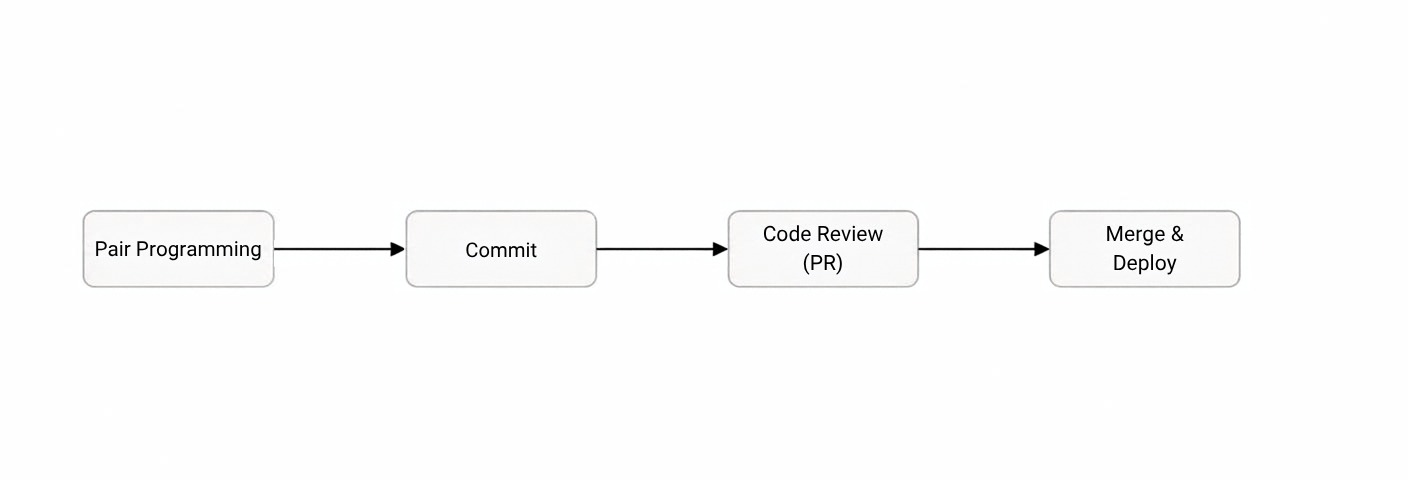
\includegraphics[width=\linewidth,keepaspectratio]{imgs/ciclo_de_vida.jpeg}
\par\smallskip
{\fontedez Fonte: elaborado pelos autores (2026), com base no Guia do Scrum [5].}
\end{figure}
\FloatBarrier

\begingroup
\small
\setlength{\tabcolsep}{3pt}
\renewcommand{\arraystretch}{1.2}
\begin{longtable}{|>{\raggedright\arraybackslash}p{\dimexpr 0.220\linewidth-2\tabcolsep-1.5\arrayrulewidth\relax}|>{\raggedright\arraybackslash}p{\dimexpr 0.780\linewidth-2\tabcolsep-1.5\arrayrulewidth\relax}|}
\hline
\textbf{Aspecto} & \textbf{Definição} \\ \hline
\endfirsthead
\textbf{Aspecto} & \textbf{Definição} \\ \hline
\endhead
Metodologia & Desenvolvimento Ágil. \\ \hline
Processo & Scrum. \\ \hline
Procedimentos & Sprint Planning, Code Review, Pair Programming, Integração Contínua, Refinamento do Backlog e Sprint Reviews. \\ \hline
Métodos & UML (Unified Modeling Language, linguagem de modelagem unificada), User Stories, Planning Poker, MoSCoW, Análise de Pontos de Função. \\ \hline
Ferramentas & Git, GitHub, Figma, VS Code, IntelliJ, Docker, Postman, Maven. \\ \hline
\end{longtable}
\noindent{\fontedez Fonte: elaborado pelos autores (2026).}
\endgroup

\subsection{ORGANIZAÇÃO DO PROJETO}

\begingroup
\small
\setlength{\tabcolsep}{4pt}
\renewcommand{\arraystretch}{1.2}
\begin{longtable}{|>{\raggedright\arraybackslash}p{\dimexpr 0.270\linewidth-2\tabcolsep-1.5\arrayrulewidth\relax}|>{\raggedright\arraybackslash}p{\dimexpr 0.430\linewidth-2\tabcolsep-1.5\arrayrulewidth\relax}|>{\raggedright\arraybackslash}p{\dimexpr 0.300\linewidth-2\tabcolsep-1.5\arrayrulewidth\relax}|}
\caption{Papéis e responsabilidades}\\
\hline
\textbf{Papel} & \textbf{Atribuições} & \textbf{Responsável} \\ \hline
\endfirsthead
\textbf{Papel} & \textbf{Atribuições} & \textbf{Responsável} \\ \hline
\endhead
Desenvolvedor Backend & Codificar o produto, codificar testes unitários, realizar refatoração. Estruturar a lógica de funcionamento do app. & Matheus Estevam, Luis, Lucas \\ \hline
Desenvolvedor Frontend & Codificar o produto, codificar testes unitários, realizar refatoração. Desenvolver a interface de usuário do app. & Rafael Laube, Mateus Fernandes \\ \hline
Documentação & Confecção dos documentos para entrega. & Bruno \\ \hline
Dono do Produto & Atualizar o escopo do produto, organizar o escopo das sprints, validar as entregas. & Monitor Daniel \\ \hline
Analista de Qualidade & Garantir a qualidade do produto, garantir o cumprimento do conceito de pronto, realizar inspeções de código. & Bernardo \\ \hline
Cliente & Validar negócio e expectativas. & Ricardo Ajax \\ \hline
\end{longtable}
\noindent{\fontedez Fonte: elaborado pelos autores (2026).}
\endgroup

\subsubsection{ANÁLISE CAUSAL}

O diagrama de Ishikawa organiza possíveis causas de um problema em categorias, relacionando-as ao efeito analisado [12]. Na Figura~\ref{fig:ishikawa}, o efeito é o abandono de atividades físicas e a desmotivação. Os ramos apresentam falta de planejamento, ausência de engajamento e falta de percepção de evolução, com suas causas específicas e os requisitos propostos para enfrentá-las:

\begin{itemize}
\item Falta de planejamento: desorganização de rotinas e divisões musculares inadequadas. Origina a necessidade de cadastro de treino (RF-03).
\item Ausência de engajamento: treinos monótonos, tédio e falta de incentivo social. Origina as conquistas (RF-22) e a submissão de desafios (RF-18).
\item Falta de percepção de evolução: dificuldade em perceber resultados rápidos. Origina o acompanhamento de métricas (RF-12).
\end{itemize}

\begin{figure}[htbp]
\centering
\caption{Diagrama de Ishikawa}
\label{fig:ishikawa}
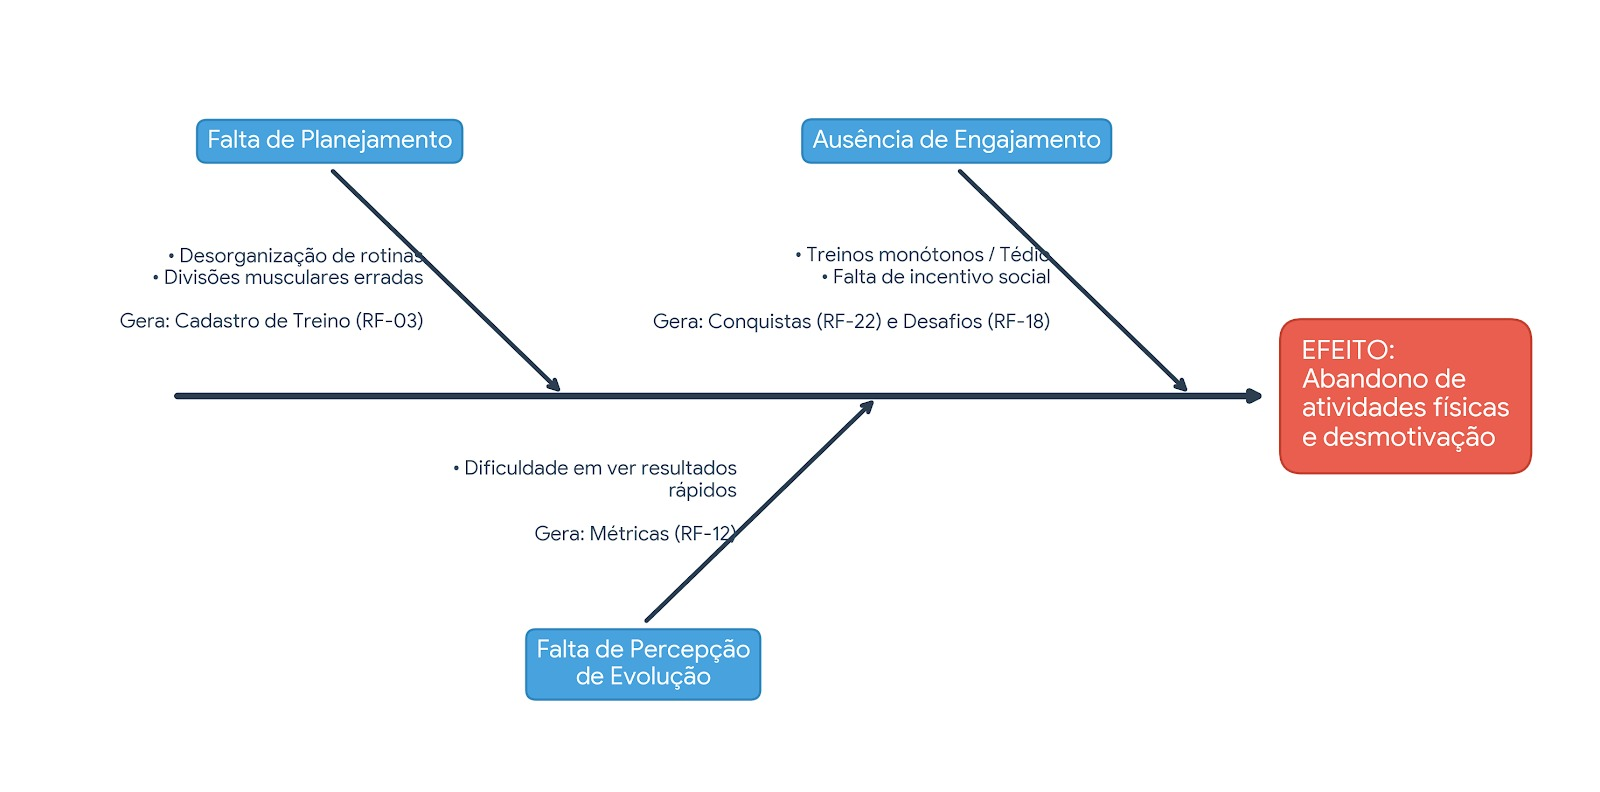
\includegraphics[width=\linewidth,keepaspectratio]{imgs/ishkawa.jpeg}
\par\smallskip
{\fontedez Fonte: elaborado pelos autores (2026), utilizando a técnica de causa e efeito descrita pela ASQ [12].}
\end{figure}
\FloatBarrier

\subsection{PLANEJAMENTO DAS FASES (SPRINTS)}

\noindent\textbf{Abreviações da tabela:} Resp.: responsáveis; \% acum.: percentual acumulado.

O percentual acumulado representa a cobertura funcional planejada, ponderada pelas estimativas preliminares do backlog, e não o progresso real de execução. RF-01 a RF-23 somam 47 unidades estimadas. As Sprints 3 a 9 acrescentam, respectivamente, 7, 6, 8, 6, 7, 7 e 6 unidades: o acumulado arredondado é 15\%, 28\%, 45\%, 57\%, 72\%, 87\% e 100\%. As Sprints 1 e 2 são preparatórias; a Sprint 10 estabiliza as entregas. RF-24 permanece fora do cálculo até receber uma estimativa. O progresso realizado deverá considerar somente funcionalidades concluídas, testadas e aceitas; as estimativas ainda não constituem uma contagem formal de PF.

\begingroup
\small
\setlength{\tabcolsep}{3pt}
\renewcommand{\arraystretch}{1.2}
\begin{longtable}{|>{\raggedright\arraybackslash}p{\dimexpr 0.090\linewidth-2\tabcolsep-1.5\arrayrulewidth\relax}|>{\raggedright\arraybackslash}p{\dimexpr 0.300\linewidth-2\tabcolsep-1.5\arrayrulewidth\relax}|>{\raggedright\arraybackslash}p{\dimexpr 0.170\linewidth-2\tabcolsep-1.5\arrayrulewidth\relax}|>{\raggedright\arraybackslash}p{\dimexpr 0.240\linewidth-2\tabcolsep-1.5\arrayrulewidth\relax}|>{\raggedright\arraybackslash}p{\dimexpr 0.110\linewidth-2\tabcolsep-1.5\arrayrulewidth\relax}|>{\raggedright\arraybackslash}p{\dimexpr 0.090\linewidth-2\tabcolsep-1.5\arrayrulewidth\relax}|}
\caption{Planejamento das sprints}\\
\hline
\textbf{Sprint} & \textbf{Produto (Entrega)} & \textbf{Período} & \textbf{Entregáveis} & \textbf{Resp.} & \textbf{\% acum.} \\ \hline
\endfirsthead
\textbf{Sprint} & \textbf{Produto (Entrega)} & \textbf{Período} & \textbf{Entregáveis} & \textbf{Resp.} & \textbf{\% acum.} \\ \hline
\endhead
1 & Definição do Produto, Documento de Visão, definição do MVP e Planejamento do Projeto. & 22/09/2026 a 27/09/2026 & Documento de visão. & Todos & 0\% \\ \hline
2 & Documento de Arquitetura, base estrutural de projeto e testes. & 28/09/2026 a 04/10/2026 & Documento de Arquitetura, estrutura base e testes, slides das apresentações. & Todos & 0\% \\ \hline
3 & Cadastro de usuário e autenticação com e-mail e senha e treinos (cadastro, listagem, alteração e exclusão de treino). & 05/10/2026 a 11/10/2026 & Backend, Banco de Dados e interfaces base. & Todos & 15\% \\ \hline
4 & Manter exercícios (cadastrar, listar, alterar, excluir e marcar exercício como realizado). Conclusão e validação do MVP com cadastro e login por e-mail e senha, treinos e exercícios. & 12/10/2026 a 18/10/2026 & Testes unitários aprovados e documentação. & Todos & 28\% \\ \hline
5 & Acompanhamento de métricas do usuário, convite de usuário administrador com e-mail. Painel administrativo: visualizar usuários ativos nos últimos 30 dias. & 19/10/2026 a 25/10/2026 & Testes unitários aprovados e documentação. & Todos & 45\% \\ \hline
6 & Painel administrativo: frequência média de treinos, ranking de treinos. & 26/10/2026 a 01/11/2026 & Testes unitários aprovados e documentação. & Todos & 57\% \\ \hline
7 & Painel administrativo: exibir os três exercícios mais realizados pelos usuários. Painel do usuário: submissão de desafios, remoção de desafios. & 02/11/2026 a 08/11/2026 & Testes unitários aprovados e documentação. & Todos & 72\% \\ \hline
8 & Criação do botão de recorde pessoal, sistema de compartilhamento comunitário. & 09/11/2026 a 15/11/2026 & Testes unitários aprovados e documentação. & Todos & 87\% \\ \hline
9 & Inspeções, streak diário, feed de atividades interativo. Integração opcional do login com o Google (RF-24, Could have), conforme a capacidade da equipe. & 16/11/2026 a 22/11/2026 & Testes unitários aprovados e documentação. & Todos & 100\% \\ \hline
10 & Estabilização e entrega: testes, correções de bugs e entrega do produto final. Validação do login com o Google (RF-24, Could have), caso implementado. & 23/11/2026 a 29/11/2026 & Entrega do produto final, documentação final e testes totais. & Todos & 100\% \\ \hline
\end{longtable}
\noindent{\fontedez Fonte: elaborado pelos autores (2026).}
\endgroup

\subsection{MATRIZ DE COMUNICAÇÃO}

\begingroup
\small
\setlength{\tabcolsep}{4pt}
\renewcommand{\arraystretch}{1.2}
\begin{longtable}{|>{\raggedright\arraybackslash}p{\dimexpr 0.250\linewidth-2\tabcolsep-1.5\arrayrulewidth\relax}|>{\raggedright\arraybackslash}p{\dimexpr 0.250\linewidth-2\tabcolsep-1.5\arrayrulewidth\relax}|>{\raggedright\arraybackslash}p{\dimexpr 0.250\linewidth-2\tabcolsep-1.5\arrayrulewidth\relax}|>{\raggedright\arraybackslash}p{\dimexpr 0.250\linewidth-2\tabcolsep-1.5\arrayrulewidth\relax}|}
\caption{Matriz de comunicação}\\
\hline
\textbf{Descrição} & \textbf{Envolvidos} & \textbf{Periodicidade} & \textbf{Produtos Gerados} \\ \hline
\endfirsthead
\textbf{Descrição} & \textbf{Envolvidos} & \textbf{Periodicidade} & \textbf{Produtos Gerados} \\ \hline
\endhead
Acompanhamento das Atividades em Andamento & Toda a equipe do projeto & Semanal & Ata de reunião, relatório de situação do projeto. \\ \hline
Acompanhamento dos Riscos, Compromissos, Ações Pendentes, Indicadores & Toda a equipe do projeto & Semanal & Relatórios focados na resolução de pendências e riscos. \\ \hline
Comunicar situação do projeto & Toda a equipe, Professor e Monitor & Diária & Alinhamentos quanto ao progresso do projeto \\ \hline
\end{longtable}
\noindent{\fontedez Fonte: elaborado pelos autores (2026).}
\endgroup

\subsection{GERENCIAMENTO DE RISCOS}

\begingroup
\small
\setlength{\tabcolsep}{3pt}
\renewcommand{\arraystretch}{1.2}
\begin{longtable}{|>{\raggedright\arraybackslash}p{\dimexpr 0.190\linewidth-2\tabcolsep-1.5\arrayrulewidth\relax}|>{\raggedright\arraybackslash}p{\dimexpr 0.160\linewidth-2\tabcolsep-1.5\arrayrulewidth\relax}|>{\raggedright\arraybackslash}p{\dimexpr 0.120\linewidth-2\tabcolsep-1.5\arrayrulewidth\relax}|>{\raggedright\arraybackslash}p{\dimexpr 0.230\linewidth-2\tabcolsep-1.5\arrayrulewidth\relax}|>{\raggedright\arraybackslash}p{\dimexpr 0.300\linewidth-2\tabcolsep-1.5\arrayrulewidth\relax}|}
\caption{Riscos}\\
\hline
\textbf{Risco} & \textbf{Fase do Projeto} & \textbf{Grau} & \textbf{Mitigação (Prevenção)} & \textbf{Contingência (Reação)} \\ \hline
\endfirsthead
\textbf{Risco} & \textbf{Fase do Projeto} & \textbf{Grau} & \textbf{Mitigação (Prevenção)} & \textbf{Contingência (Reação)} \\ \hline
\endhead
Atraso nas entregas devido ao ciclo curto de 1 semana & Todas as Sprints & Alto & Realizar reuniões de Sprint Planning rigorosas. & Não negociar o aumento da duração da Sprint. As tarefas não concluídas devem ser interrompidas, retornar para o backlog e ser replanejadas para entrega na Sprint imediatamente seguinte. \\ \hline
Abandono/Saída de membro da equipe & Todas as Sprints & Baixo & Fomentar a prática de Pair Programming para evitar que apenas uma pessoa saiba mexer numa parte do código e manter a documentação sempre atualizada. & Redistribuir imediatamente as tarefas críticas pelos restantes membros da equipe e reportar ao P.O. (Monitor Daniel) para reduzir a carga de trabalho (story points) planejada para as Sprints seguintes. \\ \hline
Falha na integração com serviços externos (Autenticação Google) & Sprints 9 e 10 (RF-24, Could have) & Médio & Iniciar os testes de requisição isoladamente via Postman antes de integrar o código ao front-end e back-end. & Manter o cadastro e login com e-mail e senha já disponíveis no MVP (CF-01 e CF-02). Replanejar a integração opcional com o Google (CF-09) sem bloquear as funcionalidades obrigatórias ou comprometer a entrega final. \\ \hline
Desalinhamento com as expectativas do cliente & Sprints de Ponto de Controle & Baixo & Envolver o cliente nas Sprint Reviews, reforçando a cada reunião o cronograma de entregas e deixando claro que o software é entregue em incrementos e ainda se encontra em fase de construção. & Agendar uma reunião extraordinária de alinhamento para relembrar os prazos estritos das Sprints, esclarecendo que qualquer nova exigência não negociada irá para o Backlog para não comprometer o prazo da Sprint atual. \\ \hline
\end{longtable}
\noindent{\fontedez Fonte: elaborado pelos autores (2026).}
\endgroup

\subsection{CRITÉRIOS DE REPLANEJAMENTO}

Os critérios de replanejamento definem os cenários críticos que inviabilizam o cronograma atual. Para o projeto MotivaFit, utilizando a metodologia Scrum, qualquer replanejamento causará o versionamento deste documento. Os critérios adotados são:

\begin{itemize}
\item Abandono da equipe por parte de algum membro, exigindo a readequação dos pontos de esforço da Sprint.
\item Alterações de Escopo: se o cliente ou o Dono do Produto solicitarem mudanças estruturais nos cenários funcionais que ultrapassem a capacidade de entrega semanal da equipe.
\item Atraso crítico em requisitos MUST: caso a equipe atrase e não consiga entregar funcionalidades obrigatórias.
\item Acumulação de Dívida Técnica (Débito Técnico): quando a métrica de débito técnico (falta de refatoração, código não documentado ou ausência de testes) atingir um nível crítico que torne a base de código insustentável, impedindo a equipe de desenvolver e integrar novas funcionalidades com segurança.
\end{itemize}


% Transcrito de Documento_Visao_MotivaFit_Completo_e_Detalhado.pdf
\clearpage
\section{PROCESSO DE DESENVOLVIMENTO DE SOFTWARE}

O fluxo de trabalho unifica a estrutura de gestão do Scrum com práticas de engenharia do eXtreme Programming (XP) [4, 5]. O gerenciamento estrutura entregas em Sprints iterativas curtas. O desenvolvimento é guiado por Testes Contínuos e Pair Programming. A esteira técnica utiliza Code Review constante entre a equipe e Integração Contínua (CI) via GitHub Actions, com aplicação contínua de princípios SOLID (responsabilidade única, aberto/fechado, substituição de Liskov, segregação de interfaces e inversão de dependência) e Clean Code no desenvolvimento em Java/Spring Boot.

A equipe não adotará a Daily Scrum, pois a disponibilidade dos integrantes impossibilita a realização de encontros diários. Essa decisão representa uma adaptação do processo em relação ao Scrum descrito em [5]. O acompanhamento das atividades e a comunicação de impedimentos ocorrerão pelos canais de comunicação do grupo e nas reuniões semanais de acompanhamento.

A Figura~\ref{fig:fluxo_de_trabalho} mostra o fluxo de trabalho no nível de gestão das entregas. Os requisitos partem do Product Backlog e são selecionados durante a Sprint Planning, formando o Sprint Backlog. Durante a Sprint de uma semana, a equipe implementa os itens selecionados, aplica os testes e realiza as revisões de código e a integração contínua descritas nesta seção. Essas práticas técnicas ocorrem dentro da etapa Sprint, embora não estejam detalhadas na imagem.

A etapa Review \& Retro reúne a avaliação da entrega e a reflexão sobre o processo. A Review verifica o resultado com os interessados; a Retrospectiva orienta ajustes para o próximo ciclo. O incremento corresponde à parte concluída do produto. Os itens pendentes ou as novas necessidades retornam ao planejamento das próximas Sprints [5].

\begin{figure}[htbp]
\centering
\caption{Fluxo de trabalho do projeto}
\label{fig:fluxo_de_trabalho}
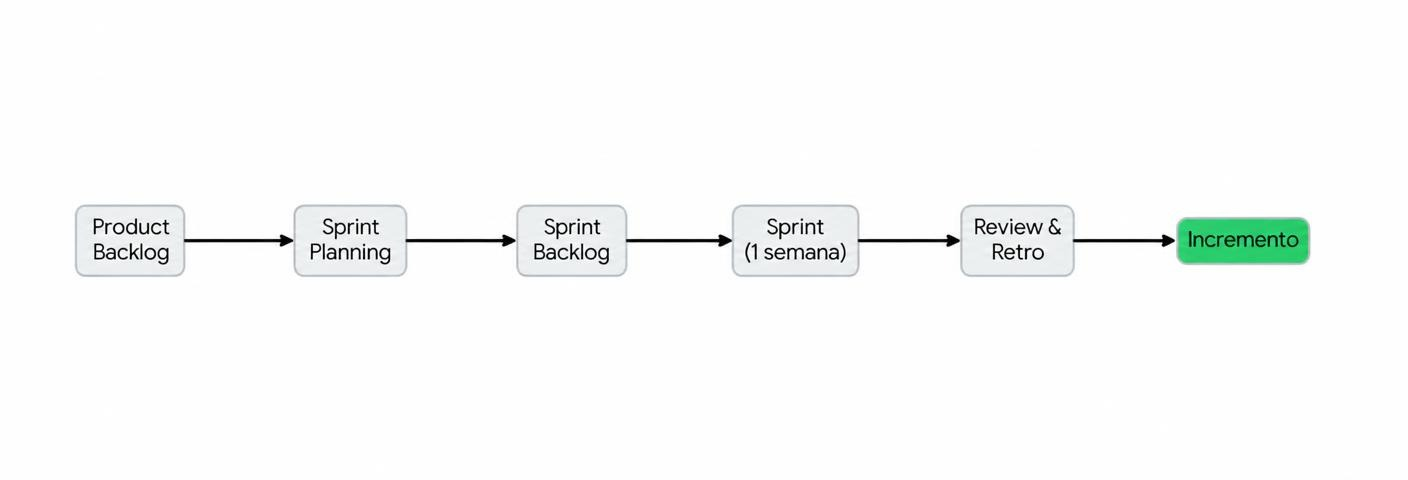
\includegraphics[width=\linewidth,keepaspectratio]{imgs/fluxo_de_trabalho.jpeg}
\par\smallskip
{\fontedez Fonte: elaborado pelos autores (2026), com base no Guia do Scrum [5].}
\end{figure}
\FloatBarrier


% Transcrito de Documento_Visao_MotivaFit_Completo_e_Detalhado.pdf
\clearpage
\section{DECLARAÇÃO DE ESCOPO DO PROJETO}

O escopo central do projeto abrange a criação de uma plataforma interativa onde o 'Atleta Amador' pode criar fichas de treino personalizadas, registrar a conclusão diária de exercícios (check-ins) e acompanhar seu progresso estatístico. Estão inclusas no escopo as lógicas de gamificação (Hexad) para recompensar a assiduidade do usuário, além de um painel administrativo para gestão global do sistema.

\subsection{BACKLOG DO PRODUTO}

A elicitação dos requisitos e a construção deste backlog foram realizadas majoritariamente por meio de brainstorming entre os membros da equipe e análise do problema, com base nas dificuldades reais de praticantes de exercícios físicos em manter a constância.

\subsubsection{CLASSIFICAÇÃO DE PRIORIDADE (MOSCOW)}

MoSCoW reúne as categorias Must have (obrigatório), Should have (importante), Could have (desejável) e Won't have (fora da entrega atual).

A priorização dos itens foi definida da seguinte forma (visão da equipe a ser validada pelo Dono do Produto (P.O., Product Owner)):

MUST (Obrigatório): Requisitos essenciais ao produto. O MVP da Sprint 4 reúne RF-01 a RF-11; RF-12 também é obrigatório para o produto, mas sua entrega está prevista para a Sprint 5, após o MVP.

SHOULD (Importante): Requisitos de alto valor agregado (como funcionalidades de gamificação e gráficos). São fundamentais para a retenção e proposta de valor do aplicativo, mas não impedem o fluxo básico de uso se entregues em um segundo momento.

COULD (Desejável): Funcionalidades que ampliam a experiência de uso, como a integração de login com o Google, mas que possuem menor prioridade e não são necessárias para a entrega do MVP. Sua implementação depende da capacidade disponível nas Sprints finais.

\subsection{PERFIS}

Teremos dois perfis de acesso, o usuário e o administrador. O usuário poderá acessar todas as funcionalidades referentes ao uso do aplicativo, ficando livre para testar as funcionalidades, enquanto o perfil administrador acompanhará as métricas e informações do aplicativo, como número de usuários, funcionalidades mais usadas e tempo médio de usuário no app, dentre outros.

\begingroup
\small
\setlength{\tabcolsep}{4pt}
\renewcommand{\arraystretch}{1.2}
\begin{longtable}{|>{\raggedright\arraybackslash}p{\dimexpr 0.333\linewidth-2\tabcolsep-1.5\arrayrulewidth\relax}|>{\raggedright\arraybackslash}p{\dimexpr 0.333\linewidth-2\tabcolsep-1.5\arrayrulewidth\relax}|>{\raggedright\arraybackslash}p{\dimexpr 0.333\linewidth-2\tabcolsep-1.5\arrayrulewidth\relax}|}
\caption{Perfis de acesso}\\
\hline
\textbf{Perfil} & \textbf{Características} & \textbf{Permissões} \\ \hline
\endfirsthead
\textbf{Perfil} & \textbf{Características} & \textbf{Permissões} \\ \hline
\endhead
Administrador & Acompanham as métricas de uso do aplicativo: quantos usuários acessaram nos últimos 30 dias, qual a frequência média de treino, quem está no topo das atividades e quais atividades estão sendo mais utilizadas. & Painel Admin (métricas). \\ \hline
Usuário & Atletas ou iniciantes em atividades físicas. Buscam registrar seus desempenhos individuais e comparar com seus amigos. & Uso do app e métricas individuais. \\ \hline
\end{longtable}
\noindent{\fontedez Fonte: elaborado pelos autores (2026).}
\endgroup

\subsection{CENÁRIOS}

\begingroup
\small
\setlength{\tabcolsep}{4pt}
\renewcommand{\arraystretch}{1.2}
\begin{longtable}{|>{\raggedright\arraybackslash}p{\dimexpr 0.150\linewidth-2\tabcolsep-1.5\arrayrulewidth\relax}|>{\raggedright\arraybackslash}p{\dimexpr 0.670\linewidth-2\tabcolsep-1.5\arrayrulewidth\relax}|>{\raggedright\arraybackslash}p{\dimexpr 0.180\linewidth-2\tabcolsep-1.5\arrayrulewidth\relax}|}
\caption{Cenários funcionais}\\
\hline
\textbf{ID} & \textbf{Cenário} & \textbf{Sprints} \\ \hline
\endfirsthead
\textbf{ID} & \textbf{Cenário} & \textbf{Sprints} \\ \hline
\endhead
CF-01 & Novo usuário cria sua conta com e-mail e senha & 3 \\ \hline
CF-02 & Usuário cadastrado deseja autenticar-se com e-mail e senha & 3 \\ \hline
CF-03 & Usuário deseja cadastrar, listar, alterar ou excluir seus treinos & 3 \\ \hline
CF-04 & Usuário deseja cadastrar, listar, alterar e excluir exercícios de um treino e registrar sua execução & 4 \\ \hline
CF-05 & Usuário já possui acesso ao sistema e deseja acompanhar sua evolução nos treinos & 5, 8 \\ \hline
CF-06 & Usuário já possui acesso ao sistema, já possui registros de exercícios, busca novos desafios e deseja comparar sua evolução com a de seu grupo de amigos & 7, 8, 9 \\ \hline
CF-07 & Administrador não possui acesso, mas pode receber um e-mail de convite para realizar seu cadastro & 5 \\ \hline
CF-08 & Administrador já tem acesso ao sistema e deseja acessar o painel de acompanhamento de métricas & 5, 6, 7 \\ \hline
CF-09 & Usuário deseja autenticar-se pelo Google como alternativa ao acesso com e-mail e senha, após a entrega do MVP & 9, 10 \\ \hline
\end{longtable}
\noindent{\fontedez Fonte: elaborado pelos autores (2026).}
\endgroup

\subsection{TABELA DE BACKLOG DO PRODUTO}

\noindent\textbf{Abreviações da tabela:} Est.: estimativa preliminar de planejamento do requisito, sem equivalência direta em horas ou contagem formal de PF; US: User Story (história de usuário); ID: identificador. O símbolo -- indica estimativa ainda não definida.

O backlog identifica cada requisito funcional pelo código RF e o cenário de uso correspondente pelo código CF. Um cenário pode reunir vários requisitos: por exemplo, CF-03 corresponde ao gerenciamento de treinos e está associado a cadastro (RF-03), listagem (RF-04), alteração (RF-05) e exclusão (RF-06). Essa identificação permite relacionar cada funcionalidade ao planejamento e aos testes.

Pontos de função (PF) são uma unidade de medida do tamanho funcional do software, considerando as funcionalidades oferecidas ao usuário, independentemente da linguagem ou tecnologia utilizada [8]. A contagem considera funções de dados e transações, como entradas, saídas e consultas, classificadas conforme sua complexidade. PF não representa diretamente horas de trabalho nem pontos de esforço da Sprint.

O MVP será concluído ao final da Sprint 4 e compreenderá o cadastro e o login com e-mail e senha, o gerenciamento de treinos e o gerenciamento e registro de exercícios. O acesso inicial está dividido em cadastro de usuário com e-mail e senha (RF-01, cenário CF-01) e autenticação com e-mail e senha (RF-02, cenário CF-02), ambos obrigatórios (Must have). O backlog atribui o valor inicial de 1 a cada requisito, totalizando 2 unidades estimadas para cadastro e autenticação. Esses valores são estimativas preliminares de planejamento; a contagem formal em PF depende do detalhamento das funções, dos dados envolvidos e da aplicação das regras de contagem [8]. O desenvolvimento dessas funcionalidades está distribuído entre as Sprints 3 e 4, com a conclusão e validação do conjunto de login, treinos e exercícios na Sprint 4, conforme os casos de teste previstos.

A integração de login com o Google corresponde ao requisito RF-24, associado ao cenário CF-09, com prioridade Could have. Está prevista para as Sprints finais: implementação na Sprint 9 e validação na Sprint 10, conforme a capacidade da equipe. O acesso com e-mail e senha permanece disponível independentemente dessa integração. A estimativa funcional de RF-24 será definida no refinamento do requisito.

\begingroup
\small
\setlength{\tabcolsep}{4pt}
\renewcommand{\arraystretch}{1.2}
\begin{longtable}{|>{\raggedright\arraybackslash}p{\dimexpr 0.17\linewidth-2\tabcolsep-1.5\arrayrulewidth\relax}|>{\raggedright\arraybackslash}p{\dimexpr 0.16\linewidth-2\tabcolsep-1.5\arrayrulewidth\relax}|>{\raggedright\arraybackslash}p{\dimexpr 0.12\linewidth-2\tabcolsep-1.5\arrayrulewidth\relax}|>{\raggedright\arraybackslash}p{\dimexpr 0.25\linewidth-2\tabcolsep-1.5\arrayrulewidth\relax}|>{\raggedright\arraybackslash}p{\dimexpr 0.3\linewidth-2\tabcolsep-1.5\arrayrulewidth\relax}|}
\caption{Backlog detalhado}\\
\hline
\textbf{Requisito} & \textbf{Planejamento} & \textbf{Tipo} & \textbf{Descrição sucinta} & \textbf{User story associada} \\ \hline
\endfirsthead
\textbf{Requisito} & \textbf{Planejamento} & \textbf{Tipo} & \textbf{Descrição sucinta} & \textbf{User story associada} \\ \hline
\endhead
RF-01\newline Cadastro com e-mail e senha & CF-01\newline Sprint 3\newline Must\newline Est.: 1 & Funcional & Criar conta com e-mail e senha. & US-01: Como visitante, quero criar minha conta com e-mail e senha para acessar o aplicativo. \\ \hline
RF-02\newline Login com e-mail e senha & CF-02\newline Sprint 3\newline Must\newline Est.: 1 & Funcional & Autenticar com e-mail e senha e rejeitar credenciais inválidas. & US-02: Como usuário cadastrado, quero entrar com e-mail e senha para acessar meus treinos. \\ \hline
RF-03\newline Cadastro de Treino & CF-03\newline Sprint 3\newline Must\newline Est.: 1 & Funcional & Cadastrar treino com nome e tipo. & US-03: Como usuário, quero cadastrar meu treino para organizar minha rotina. \\ \hline
RF-04\newline Listagem de Treinos & CF-03\newline Sprint 3\newline Must\newline Est.: 2 & Funcional & Listar os treinos do usuário e permitir adicionar treinos já montados. & US-04: Como usuário, quero visualizar meus treinos e adicionar treinos já montados para organizar minhas opções. \\ \hline
RF-05\newline Alteração de Treino & CF-03\newline Sprint 3\newline Must\newline Est.: 1 & Funcional & Alterar nome e tipo de treino. & US-05: Como usuário, quero alterar meu treino para adaptar minha rotina. \\ \hline
RF-06\newline Exclusão de Treino & CF-03\newline Sprint 3\newline Must\newline Est.: 1 & Funcional & Excluir treino do usuário. & US-06: Como usuário, quero excluir um treino para remover rotinas que não utilizo. \\ \hline
RF-07\newline Cadastrar Exercício no treino & CF-04\newline Sprint 4\newline Must\newline Est.: 1 & Funcional & Adicionar exercício predefinido a um treino e definir metas. & US-07: Como usuário, quero adicionar exercícios e metas ao treino para planejar a sessão. \\ \hline
RF-08\newline Listar Exercícios & CF-04\newline Sprint 4\newline Must\newline Est.: 2 & Funcional & Listar exercícios e metas de um treino. & US-08: Como usuário, quero consultar exercícios e metas para executar meu treino. \\ \hline
RF-09\newline Alterar Exercício & CF-04\newline Sprint 4\newline Must\newline Est.: 1 & Funcional & Editar informações de exercício vinculado a treino. & US-09: Como usuário, quero ajustar as metas do exercício para adaptar meu treino. \\ \hline
RF-10\newline Excluir Exercício & CF-04\newline Sprint 4\newline Must\newline Est.: 1 & Funcional & Excluir exercício de um treino. & US-10: Como usuário, quero remover um exercício para atualizar minha rotina. \\ \hline
RF-11\newline Registrar Exercício Realizado & CF-04\newline Sprint 4\newline Must\newline Est.: 1 & Funcional & Registrar execução, carga, repetições, séries e tempo. & US-11: Como usuário, quero registrar a execução dos exercícios para manter meu histórico. \\ \hline
RF-12\newline Métricas de evolução & CF-05\newline Sprint 5\newline Must\newline Est.: 2 & Funcional & Exibir indicadores de desempenho e evolução. & US-12: Como usuário, quero acompanhar minhas métricas para perceber minha evolução. \\ \hline
RF-13\newline Convite admin por email & CF-07\newline Sprint 5\newline Could\newline Est.: 3 & Funcional & Enviar convite por e-mail para novo administrador. & US-13: Como superusuário, quero convidar administradores para delegar a gestão do sistema. \\ \hline
RF-14\newline Usuários ativos (Admin) & CF-08\newline Sprint 5\newline Should\newline Est.: 3 & Funcional & Exibir quantidade de usuários ativos nos últimos 30 dias. & US-14: Como administrador, quero consultar usuários ativos para acompanhar a adesão. \\ \hline
RF-15\newline Frequência média (Admin) & CF-08\newline Sprint 6\newline Should\newline Est.: 3 & Funcional & Exibir frequência média de treinos por semana e usuário. & US-15: Como administrador, quero consultar a frequência média para acompanhar a constância. \\ \hline
RF-16\newline Ranking usuários (Admin) & CF-08\newline Sprint 6\newline Should\newline Est.: 3 & Funcional & Exibir os dez usuários com maior tempo de treino nos últimos 30 dias. & US-16: Como administrador, quero consultar o ranking para acompanhar a atividade dos usuários. \\ \hline
RF-17\newline Exercícios + feitos (Admin) & CF-08\newline Sprint 7\newline Should\newline Est.: 3 & Funcional & Exibir os três exercícios mais realizados nos últimos 30 dias. & US-17: Como administrador, quero consultar exercícios mais realizados para conhecer o uso. \\ \hline
RF-18\newline Submissão de desafios & CF-06\newline Sprint 7\newline Must\newline Est.: 3 & Funcional & Criar desafios entre amigos com exercícios, metas e prazo. & US-18: Como usuário, quero propor desafios para incentivar meu grupo de amigos. \\ \hline
RF-19\newline Remoção de desafios & CF-06\newline Sprint 7\newline Must\newline Est.: 1 & Funcional & Remover desafio criado pelo usuário. & US-19: Como usuário, quero remover meus desafios para manter as propostas atualizadas. \\ \hline
RF-20\newline PR - Recorde Pessoal & CF-05\newline Sprint 8\newline Must\newline Est.: 2 & Funcional & Acompanhar metas de recordes pessoais no exercício. & US-20: Como usuário, quero acompanhar meus recordes pessoais para perceber minha evolução. \\ \hline
RF-21\newline Partilha de resultados & CF-06\newline Sprint 8\newline Should\newline Est.: 5 & Funcional & Compartilhar resultados em espaço comunitário público. & US-21: Como usuário, quero compartilhar meus resultados para motivar a comunidade. \\ \hline
RF-22\newline Conquistas (Streak) & CF-06\newline Sprint 9\newline Must\newline Est.: 2 & Funcional & Exibir conquistas de assiduidade no perfil. & US-22: Como usuário, quero visualizar minhas conquistas para reconhecer minha constância. \\ \hline
RF-23\newline Feed interativo & CF-06\newline Sprint 9\newline Should\newline Est.: 4 & Funcional & Permitir grupos por convite e interação com resultados diários. & US-23: Como usuário, quero curtir e comentar resultados do meu grupo para incentivar meus amigos. \\ \hline
RF-24\newline Login com Google & CF-09\newline Sprint 9, 10\newline Could\newline Est.: -- & Funcional & Oferecer autenticação opcional com Google após o MVP. & US-24: Como usuário, quero entrar com Google como alternativa para facilitar meu acesso. \\ \hline
\end{longtable}
\noindent{\fontedez Fonte: elaborado pelos autores (2026).}
\endgroup

\subsubsection{DESCRIÇÃO DOS REQUISITOS}

Todos os requisitos abaixo são do tipo funcional. Os identificadores RF correspondem aos cenários CF apresentados na tabela de backlog.

\begin{description}
\item[RF-01] Permitir ao usuário não autenticado criar sua conta no sistema informando e-mail e senha. Requisito obrigatório para o MVP, associado ao cenário CF-01.

\item[RF-02] Permitir ao usuário cadastrado acessar o sistema com e-mail e senha válidos e impedir o acesso com credenciais inválidas. Requisito obrigatório para o MVP, associado ao cenário CF-02.

\item[RF-03] O usuário adiciona o seu novo treino, definindo o nome e tipo de treino (musculação ou aeróbico).

\item[RF-04] O usuário irá visualizar o catálogo de treinos dele, permitindo também adicionar treinos já montados (basta o usuário adicionar na sua lista).

\item[RF-05] Permite ao usuário fazer alteração no treino (nome e tipo de treino: musculação ou aeróbico).

\item[RF-06] Permite ao usuário remover um treino da sua lista de treinos.

\item[RF-07] Permite ao usuário cadastrar um novo exercício dentro de um treino, definindo a meta de tempo, repetições e/ou carga deste exercício, além do pace para corrida. Essas metas ficam em um campo de texto, onde o usuário digita a meta. Esse exercício já está predefinido na tabela de exercícios, de forma que o usuário não consegue criar o seu exercício.

\item[RF-08] Listar os exercícios de um treino (exibir o nome do exercício e suas metas).

\item[RF-09] Permite ao usuário a edição e atualização das informações de um exercício já cadastrado em um treino.

\item[RF-10] Permite ao usuário remover um exercício da sua lista de exercícios de um treino.

\item[RF-11] Permite ao usuário registrar a execução de um exercício em seu treino, registrando meta de carga, de repetições, de séries e tempo de execução.

\item[RF-12] O usuário pode visualizar indicadores de desempenho e evolução física ao longo do tempo.

\item[RF-13] Permite ao superusuário enviar um convite de novo administrador pelo e-mail do novo administrador.

\item[RF-14] Exibe a quantidade de usuários ativos nos últimos 30 dias.

\item[RF-15] Exibe a frequência média de treinos/semana/usuário.

\item[RF-16] No painel do administrador, exibe o ranking dos usuários ativos nos últimos 30 dias, listados por maior tempo de treino (top 10).

\item[RF-17] No painel do administrador, exibe os 3 exercícios mais realizados pelos usuários nos últimos 30 dias.

\item[RF-18] No painel do usuário, criar uma lista de exercícios entre amigos para realizarem dentro de um prazo de tempo. Definindo, para cada exercício, metas de carga, repetições, séries ou tempo de exercício.

\item[RF-19] Permite ao usuário remover um desafio criado.

\item[RF-20] Opção para a criação de um acompanhamento sobre a evolução do usuário em suas metas de recordes pessoais (campo de texto no exercício).

\item[RF-21] Local público para compartilhar os resultados dos usuários para fazer com que eles continuem se motivando.

\item[RF-22] Conquistas visuais no perfil de cada usuário para que eles possam mostrar o seu empenho nos seus treinos.

\item[RF-23] Criação de pequenos grupos de treino onde os membros podem curtir, comentar e celebrar os resultados diários uns dos outros, fortalecendo as relações (entrada por meio de convite).

\item[RF-24] Integrar a autenticação com o Google como alternativa ao login com e-mail e senha. Requisito Could have, associado ao cenário CF-09, previsto para implementação e validação nas Sprints 9 e 10 conforme a capacidade da equipe, após a entrega do MVP. A integração não substitui o acesso com e-mail e senha.

\end{description}

\subsection{MATRIZ DE RASTREABILIDADE}

\begingroup
\small
\setlength{\tabcolsep}{4pt}
\renewcommand{\arraystretch}{1.2}
\begin{longtable}{|>{\raggedright\arraybackslash}p{\dimexpr 0.22\linewidth-2\tabcolsep-1.5\arrayrulewidth\relax}|>{\raggedright\arraybackslash}p{\dimexpr 0.16\linewidth-2\tabcolsep-1.5\arrayrulewidth\relax}|>{\raggedright\arraybackslash}p{\dimexpr 0.17\linewidth-2\tabcolsep-1.5\arrayrulewidth\relax}|>{\raggedright\arraybackslash}p{\dimexpr 0.3\linewidth-2\tabcolsep-1.5\arrayrulewidth\relax}|>{\raggedright\arraybackslash}p{\dimexpr 0.15\linewidth-2\tabcolsep-1.5\arrayrulewidth\relax}|}
\caption{Matriz de rastreabilidade}\\
\hline
\textbf{Problema / cenário} & \textbf{Perfil} & \textbf{Requisitos} & \textbf{Testes planejados} & \textbf{Métrica} \\ \hline
\endfirsthead
\textbf{Problema / cenário} & \textbf{Perfil} & \textbf{Requisitos} & \textbf{Testes planejados} & \textbf{Métrica} \\ \hline
\endhead
Acesso (CF-01, CF-02) & Usuário & RF-01, RF-02 & T1, T2, T3, T22 & M2 \\ \hline
Organização (CF-03) & Usuário & RF-03 a RF-06 & T4 a T7, T14 & Uso / Throughput \\ \hline
Personalização (CF-04) & Free Spirit & RF-07 a RF-10 & T15 a T18 & M3 \\ \hline
Registro (CF-04) & Usuário & RF-11 & T8 & Uso / M3 \\ \hline
Evolução (CF-05) & Achiever & RF-12, RF-20 & T9, T19 & Uso / Throughput \\ \hline
Convite (CF-07) & Superusuário & RF-13 & A detalhar antes da Sprint 5 & M2 \\ \hline
Gestão (CF-08) & Administrador & RF-14 a RF-17 & T11 (acesso); testes funcionais a detalhar antes das Sprints 5 a 7 & Throughput \\ \hline
Desafios (CF-06) & Disruptor & RF-18, RF-19 & A detalhar antes da Sprint 7 & Uso \\ \hline
Compartilhamento (CF-06) & Philanthropist & RF-21 & A detalhar antes da Sprint 8 & Uso \\ \hline
Conquistas (CF-06) & Player & RF-22 & T10 & Uso \\ \hline
Interação (CF-06) & Socialiser & RF-23 & A detalhar antes da Sprint 9 & Uso \\ \hline
Acesso alternativo (CF-09) & Usuário & RF-24 & T12, T13, T21, T22 & M2 \\ \hline
Usabilidade do MVP & Usuário & RF-01 a RF-11 & T20 & Conclusão das tarefas \\ \hline
\end{longtable}
\noindent{\fontedez Fonte: elaborado pelos autores (2026).}
\endgroup

% GQM e fichas conforme Documento_Visao_MotivaFit_Final_Com_Diagrama.pdf.
\clearpage
\section{MÉTRICAS E MEDIÇÕES}

Para assegurar a saúde e a transparência do projeto, aplicamos a abordagem GQM (Goal-Question-Metric, objetivo--questão--métrica) estruturada para garantir rastreabilidade entre as metas de negócio e as métricas operacionais coletadas [6].

\subsection{O QUADRO GQM ESTRUTURADO E QUESTÕES}

Os códigos G, Q e M identificam, respectivamente, objetivos (Goals), questões (Questions) e métricas (Metrics).

A tabela utiliza o padrão explícito do framework GQM (Analisar / com o propósito de / com respeito a / do ponto de vista de / no contexto de) e o relaciona diretamente às respectivas questões e métricas.

\begingroup
\small
\setlength{\tabcolsep}{4pt}
\renewcommand{\arraystretch}{1.2}
\begin{longtable}{|>{\raggedright\arraybackslash}p{\dimexpr 0.070\linewidth-2\tabcolsep-1.5\arrayrulewidth\relax}|>{\raggedright\arraybackslash}p{\dimexpr 0.470\linewidth-2\tabcolsep-1.5\arrayrulewidth\relax}|>{\raggedright\arraybackslash}p{\dimexpr 0.250\linewidth-2\tabcolsep-1.5\arrayrulewidth\relax}|>{\raggedright\arraybackslash}p{\dimexpr 0.210\linewidth-2\tabcolsep-1.5\arrayrulewidth\relax}|}
\caption{Quadro GQM de acompanhamento do projeto}\\
\hline
\textbf{ID} & \textbf{Objetivo Estruturado (Goal)} & \textbf{Questão (Question)} & \textbf{Métrica (Metric)} \\ \hline
\endfirsthead
\textbf{ID} & \textbf{Objetivo Estruturado (Goal)} & \textbf{Questão (Question)} & \textbf{Métrica (Metric)} \\ \hline
\endhead
G1 & Analisar o processo de desenvolvimento com o propósito de avaliar a cadência de entrega com respeito a produtividade da equipe do ponto de vista de gerenciamento de projeto no contexto das Sprints semanais do MotivaFit. & Q1: Qual a cadência de entrega da equipe por Sprint? & M1: Throughput (Vazão) de Issues. \\ \hline
G2 & Analisar o produto gerado com o propósito de avaliar a estabilidade do software com respeito a ocorrência de falhas do ponto de vista de qualidade no contexto das entregas contínuas do MotivaFit. & Q2: Qual a estabilidade do software entregue na Sprint? & M2: Densidade de Defeitos. \\ \hline
G3 & Analisar o código fonte com o propósito de garantir a blindagem contra regressões com respeito a testes automatizados do ponto de vista de engenharia de software no contexto da integração contínua do MotivaFit. & Q3: O código em produção está adequadamente coberto por testes? & M3: Percentual de Cobertura. \\ \hline
G4 & Analisar a base de código com o propósito de controlar a manutenibilidade com respeito a débito técnico do ponto de vista de desenvolvimento no contexto do repositório do projeto. & Q4: Qual o nível de dívida técnica acumulada no código da aplicação? & M4: Dívida Técnica. \\ \hline
\end{longtable}
\noindent{\fontedez Fonte: elaborado pelos autores (2026).}
\endgroup

\subsection{FICHAS DE DETALHAMENTO DAS MÉTRICAS (5W1H, ESCALAS E ANÁLISES)}

5W1H reúne seis perguntas: What (o quê), Why (por quê), Who (quem), Where (onde), When (quando) e How (como).

\textbf{MÉTRICA 1 (M1): THROUGHPUT (VAZÃO) DE ISSUES POR SPRINT}

\begingroup
\small
\setlength{\tabcolsep}{4pt}
\renewcommand{\arraystretch}{1.2}
\begin{longtable}{|>{\raggedright\arraybackslash}p{\dimexpr 0.310\linewidth-2\tabcolsep-1.5\arrayrulewidth\relax}|>{\raggedright\arraybackslash}p{\dimexpr 0.690\linewidth-2\tabcolsep-1.5\arrayrulewidth\relax}|}
\hline
\textbf{Campo} & \textbf{Detalhamento} \\ \hline
\endfirsthead
\textbf{Campo} & \textbf{Detalhamento} \\ \hline
\endhead
Definição & Quantidade de histórias (issues) concluídas (Done) ao final de cada iteração. \\ \hline
What (O quê) & Número de issues encerradas por Sprint. \\ \hline
Why (Por quê) & Identificar a cadência de entrega para evitar sobrecarga ou ociosidade no time. \\ \hline
Who (Quem) & Analista de Qualidade e Desenvolvedores. \\ \hline
Where (Onde) & Board do GitHub Projects (Aba 'Done'). \\ \hline
When (Quando) & Ao final de cada Sprint (durante a Review). \\ \hline
Cálculo / How (Como) & Somatório simples absoluto das tarefas movidas para a coluna de finalizadas no período. \\ \hline
Escala de unidade & issues / sprint (número inteiro). \\ \hline
Valor esperado & 4 a 6 tarefas por Sprint. Justificativa: baseado na capacidade atual de horas da equipe (estimada via Planning Poker para as \mbox{aproximadamente 14 horas} disponíveis semanais por membro). \\ \hline
Forma de análise & Gráfico de tendência (Controle de Vazão / Burn-up) analisado durante a Retrospectiva. Se o valor ficar abaixo da meta por duas Sprints, o escopo do backlog deve ser renegociado com o cliente. \\ \hline
\end{longtable}
\noindent{\fontedez Fonte: elaborado pelos autores (2026).}
\endgroup

\textbf{MÉTRICA 2 (M2): DENSIDADE DE DEFEITOS}

\begingroup
\small
\setlength{\tabcolsep}{4pt}
\renewcommand{\arraystretch}{1.2}
\begin{longtable}{|>{\raggedright\arraybackslash}p{\dimexpr 0.310\linewidth-2\tabcolsep-1.5\arrayrulewidth\relax}|>{\raggedright\arraybackslash}p{\dimexpr 0.690\linewidth-2\tabcolsep-1.5\arrayrulewidth\relax}|}
\hline
\textbf{Campo} & \textbf{Detalhamento} \\ \hline
\endfirsthead
\textbf{Campo} & \textbf{Detalhamento} \\ \hline
\endhead
Definição & Relação matemática entre os defeitos válidos registrados e o volume de entregas (issues fechadas). \\ \hline
What (O quê) & Falhas de código ou de regras de negócio identificadas. \\ \hline
Why (Por quê) & Avaliar se a velocidade de entrega não está gerando instabilidade na aplicação. \\ \hline
Who (Quem) & Analista de Qualidade (registro) e Equipe (resolução). \\ \hline
Where (Onde) & Issues do repositório no GitHub (filtradas pela label 'bug'). \\ \hline
When (Quando) & Fechamento de cada Sprint e eventos de Release. \\ \hline
Cálculo / How (Como) & D = (Nº de Bugs registrados na Sprint) / (Nº de Issues concluídas na Sprint). \\ \hline
Escala de unidade & bugs / issue (número decimal). \\ \hline
Valor esperado & $\leq$ 0,2 bugs/issue. \\ \hline
Forma de análise & Comparação direta com o teto de 0,2. Se o indicador ultrapassar esse limite, a Sprint subsequente deve travar o desenvolvimento de novas features e focar obrigatoriamente na resolução de bugs (hardening). \\ \hline
\end{longtable}
\noindent{\fontedez Fonte: elaborado pelos autores (2026).}
\endgroup

\textbf{MÉTRICA 3 (M3): PERCENTUAL DE COBERTURA DE TESTES (COVERAGE)}

\begingroup
\small
\setlength{\tabcolsep}{4pt}
\renewcommand{\arraystretch}{1.2}
\begin{longtable}{|>{\raggedright\arraybackslash}p{\dimexpr 0.310\linewidth-2\tabcolsep-1.5\arrayrulewidth\relax}|>{\raggedright\arraybackslash}p{\dimexpr 0.690\linewidth-2\tabcolsep-1.5\arrayrulewidth\relax}|}
\hline
\textbf{Campo} & \textbf{Detalhamento} \\ \hline
\endfirsthead
\textbf{Campo} & \textbf{Detalhamento} \\ \hline
\endhead
Definição & Proporção de linhas úteis de código validadas e testadas pelos scripts automatizados na esteira de integração. \\ \hline
What (O quê) & Métrica de Line Coverage da aplicação global. \\ \hline
Why (Por quê) & Garantir que refatorações não quebrem as lógicas de gamificação e treinos existentes. \\ \hline
Who (Quem) & Desenvolvedores responsáveis pelos testes e QA (Quality Assurance, garantia da qualidade) responsável pela auditoria. \\ \hline
Where (Onde) & Logs do GitHub Actions e painel de validação de PR. \\ \hline
When (Quando) & A cada abertura e atualização de Pull Request (PR) para as branches principais. \\ \hline
Cálculo / How (Como) & C = [(Linhas Cobertas Backend + Linhas Cobertas Frontend) / (Total de Linhas Backend + Total de Linhas Frontend)] × 100. \\ \hline
Escala de unidade & Porcentagem (\%). \\ \hline
Valor esperado & $\geq$ 70\%. Justificativa: limiar de convenção interna para balancear estabilidade e agilidade na prototipagem inicial. \\ \hline
Forma de análise & Ação automatizada bloqueante no CI. Pull Requests que reduzam o percentual global para baixo da meta de 70\% não poderão ser mesclados (merged) sob nenhuma hipótese. \\ \hline
\end{longtable}
\noindent{\fontedez Fonte: elaborado pelos autores (2026).}
\endgroup

\textbf{MÉTRICA 4 (M4): DÍVIDA TÉCNICA (DÉBITO TÉCNICO)}

\begingroup
\small
\setlength{\tabcolsep}{4pt}
\renewcommand{\arraystretch}{1.2}
\begin{longtable}{|>{\raggedright\arraybackslash}p{\dimexpr 0.310\linewidth-2\tabcolsep-1.5\arrayrulewidth\relax}|>{\raggedright\arraybackslash}p{\dimexpr 0.690\linewidth-2\tabcolsep-1.5\arrayrulewidth\relax}|}
\hline
\textbf{Campo} & \textbf{Detalhamento} \\ \hline
\endfirsthead
\textbf{Campo} & \textbf{Detalhamento} \\ \hline
\endhead
Definição & Medição contínua de violações de boas práticas de desenvolvimento e arquitetura, incluindo bad smells, código duplicado e alto acoplamento [7]. \\ \hline
What (O quê) & Complexidade Ciclomática e Code Smells. \\ \hline
Why (Por quê) & Prevenir o envelhecimento precoce e a insustentabilidade a longo prazo da base de código. \\ \hline
Who (Quem) & Todos os membros da equipe de engenharia. \\ \hline
Where (Onde) & Dashboard de monitoramento da ferramenta de análise estática (ex: SonarQube). \\ \hline
When (Quando) & Escaneamento diário executado automaticamente pela pipeline. \\ \hline
Cálculo / How (Como) & Varredura do AST (Abstract Syntax Tree, árvore de sintaxe abstrata) da aplicação identificando anti-patterns pré-configurados. \\ \hline
Escala de unidade & Número absoluto de Code Smells e avaliação em letras (A, B, C, D) para manutenibilidade. \\ \hline
Valor esperado & Zero (0) falhas críticas / Classificação 'A'. \\ \hline
Forma de análise & Acompanhamento visual via badge no repositório. O aparecimento de qualquer defeito de nível 'Crítico' ou 'Blocker' instaura prioridade máxima de refatoração para a dupla de desenvolvimento (Pair Programming) do dia. \\ \hline
\end{longtable}
\noindent{\fontedez Fonte: elaborado pelos autores (2026).}
\endgroup


% Transcrito de Documento_Visao_MotivaFit_Completo_e_Detalhado.pdf
\clearpage
\section{TESTES DE SOFTWARE}

A estratégia de qualidade foca em garantir uma experiência fluida e livre de falhas lógicas. A abordagem engloba testes unitários rigorosos (especialmente para a lógica de pontuação e serviços do back-end), testes funcionais de integração da API (Application Programming Interface, interface de programação de aplicações) e avaliações de desempenho. O objetivo é assegurar não apenas o funcionamento correto, mas também garantir que as interfaces respondam rapidamente.

\subsection{ESTRATÉGIA DE TESTES}

Níveis de testes abordados:

\begin{itemize}
\item Unitário: Testes isolados de funções e componentes.

\item Integração: Testes da comunicação entre módulos, com foco na interação das rotas da API com a base de dados (PostgreSQL) e na integração das telas do frontend com os endpoints do backend.

\item Sistema: Testes que simulam o fluxo completo do usuário, desde a interação na interface móvel até a resposta do servidor e persistência dos dados.

\end{itemize}

Tipos de testes abordados: o foco principal reside nos testes funcionais: validação das regras de negócio (criação de treinos, evolução de cargas), fluxos de autenticação com e-mail e senha no MVP e, nas Sprints finais, login opcional com o Google e operações de CRUD (Create, Read, Update, Delete: criar, consultar, atualizar e excluir) no sistema. Adicionalmente, são planejados testes não funcionais focados na usabilidade da interface móvel e na sua adaptação a diferentes telas.

Ambientes de testes usados:

O processo de testes obedece à política de branches e commits estabelecida para o projeto no GitHub:

\begin{itemize}
\item Ambiente Local: ambiente utilizado pela equipe de desenvolvimento para a criação e execução dos testes na respectiva branch da funcionalidade antes de solicitar a integração.

\item Ambiente de Integração Contínua (CI): ao abrir um Pull Request para a branch principal, os fluxos do GitHub Actions são acionados automaticamente, executando os testes unitários e de integração em containers Docker. O merge só é autorizado se toda a pipeline de testes for aprovada sem falhas.

\end{itemize}

\textbf{FORMAS DE ANÁLISE DOS TESTES PROPOSTOS}

Os testes são avaliados através dos relatórios de execução local e dos logs de execução do GitHub Actions. Em caso de falha, o Analista de Qualidade (Bernardo) examina o erro em conjunto com os desenvolvedores responsáveis pela funcionalidade, garantindo o reparo e acompanhando a correção através de inspeções de código até a nova aprovação dos testes.

\textbf{RESULTADOS OBTIDOS}

Até esta revisão, os casos estão planejados e não há resultados de execução ou evidências registrados neste documento. O registro de execução da seção 6.2 apresenta essa situação explicitamente, com zero ciclos executados. Cada caso de teste possui um resultado esperado (previsto), detalhado no roteiro de testes (seção 6.2). Qualquer divergência frente ao comportamento real (realizado) da aplicação é identificada como um defeito. Esse defeito deve ser reparado e o ciclo de teste repetido até que o resultado realizado corresponda ao previsto (Previsto = Realizado), atingindo o critério de aprovação do caso executado. Casos apenas planejados não constituem evidência de ausência de defeitos.

\subsection{ROTEIRO DE TESTE}

Os códigos T identificam os casos de teste.

O roteiro documenta os cenários de validação planejados (Test Plan). O resultado obtido, a referência da evidência, os reparos e o número de ciclos devem ser atualizados no registro de execução após cada teste. Evidências externas devem ser identificadas por caminho ou URL (Uniform Resource Locator, endereço de um recurso), versão do código e data. Casos apenas planejados não garantem ausência de defeitos, mas estabelecem o critério de sucesso.

O roteiro é organizado em duas tabelas vinculadas pelo ID: planejamento (tipo, nível, pré-condições e resultado previsto) e execução (resultado obtido, evidência, reparos e ciclos). O detalhamento apresenta o objetivo e, nos novos casos, os procedimentos. T2 e T3 validam e-mail e senha do MVP; não testam a senha do Google. O consentimento cancelado é tratado em T13, tokens inválidos ou expirados em T21 e acesso sem sessão em T22.

Os casos T1 a T8, T14 a T18 e T22 devem ser executados nas Sprints 3 e 4; T20 valida o conjunto do MVP na Sprint 4. T9 será executado na Sprint 5, T19 na Sprint 8 e T10 na Sprint 9. T11 acompanha a entrega das funcionalidades administrativas. T12, T13 e T21 dependem da implementação de RF-24 nas Sprints 9 e 10. Os casos funcionais ainda não detalhados de RF-13 a RF-19, RF-21 e RF-23 deverão ser definidos antes da Sprint de implementação de cada requisito, com atualização da matriz. O teste de acesso T11 não substitui os testes funcionais do painel administrativo.

\begingroup
\small
\setlength{\tabcolsep}{4pt}
\renewcommand{\arraystretch}{1.2}
\begin{longtable}{|>{\raggedright\arraybackslash}p{\dimexpr 0.19\linewidth-2\tabcolsep-1.5\arrayrulewidth\relax}|>{\raggedright\arraybackslash}p{\dimexpr 0.15\linewidth-2\tabcolsep-1.5\arrayrulewidth\relax}|>{\raggedright\arraybackslash}p{\dimexpr 0.12\linewidth-2\tabcolsep-1.5\arrayrulewidth\relax}|>{\raggedright\arraybackslash}p{\dimexpr 0.24\linewidth-2\tabcolsep-1.5\arrayrulewidth\relax}|>{\raggedright\arraybackslash}p{\dimexpr 0.3\linewidth-2\tabcolsep-1.5\arrayrulewidth\relax}|}
\caption{Planejamento dos testes}\\
\hline
\textbf{ID / nome} & \textbf{Tipo} & \textbf{Nível} & \textbf{Pré-condições} & \textbf{Resultado previsto} \\ \hline
\endfirsthead
\textbf{ID / nome} & \textbf{Tipo} & \textbf{Nível} & \textbf{Pré-condições} & \textbf{Resultado previsto} \\ \hline
\endhead
T1 Cadastro de usuário com e-mail e senha & Funcional & Integração & Usuário ainda não cadastrado; acesso à tela de cadastro; e-mail e senha válidos para o cadastro & A conta e o perfil do usuário são criados. O usuário pode acessar a tela de login para se autenticar com o e-mail e a senha cadastrados \\ \hline
T2 Login com credencial válida & Funcional & Sistema & Usuário previamente cadastrado; e-mail e senha válidos & O sistema autentica o usuário e exibe a tela principal correspondente ao perfil \\ \hline
T3 Login com dados inválidos & Funcional / Segurança & Sistema & Usuário cadastrado; senha ou e-mail incorreto & O sistema nega o acesso e apresenta uma mensagem clara, sem revelar informação sensível \\ \hline
T4 Cadastro de treino personalizado & Funcional & Integração & Usuário autenticado; acesso ao formulário de treino; nome e tipo válidos & O treino é validado, salvo no banco de dados e exibido na lista de treinos do usuário \\ \hline
T5 Validação de treino incompleto & Funcional / Validação & Integração & Usuário autenticado; acesso à tela de criação de treino & O sistema impede o salvamento e informa quais campos precisam ser preenchidos. Nenhum registro incompleto é criado \\ \hline
T6 Alteração de treino existente & Funcional & Integração & Usuário autenticado; existência de um treino salvo & As alterações são salvas e aparecem corretamente na visualização do treino \\ \hline
T7 Exclusão de treino & Funcional & Sistema & Usuário autenticado; existência de treino salvo & O sistema solicita confirmação, exclui o treino após a confirmação e remove o item da listagem. Se o usuário cancelar, o treino permanece salvo \\ \hline
T8 Registro de exercício realizado & Funcional & Integração & Usuário autenticado; existência de treino cadastrado & O exercício é marcado como realizado, o histórico é atualizado e as informações são persistidas pelo banco de dados \\ \hline
T9 Atualização de métricas de evolução & Funcional & Sistema & Usuário autenticado; existência de exercícios realizados com datas e cargas registradas & Os gráficos e indicadores apresentam os dados correspondentes aos exercícios realizados \\ \hline
T10 Pontuação e conquista por assiduidade & Funcional / Gamificação & Integração & Usuário autenticado; critérios de conquista definidos; registros de assiduidade preparados & O sistema exibe a conquista no perfil somente quando os critérios de assiduidade são atingidos \\ \hline
T11 Restrição do painel de admin & Não funcional / Segurança & Integração & Existência de um usuário comum e um usuário administrador & O usuário comum não consegue acessar o painel administrativo. O administrador consegue acessá-lo normalmente \\ \hline
T12 Login com google & Funcional / Autenticação & Integração & Integração com o Google implementada e configurada; conta Google válida; serviço de autenticação disponível & Após autorização e validação da autenticação com o Google, o usuário acessa o sistema com seu perfil. O login com e-mail e senha permanece disponível \\ \hline
T13 Falha ou cancelamento no login com google & Funcional / Segurança & Integração & Integração com o Google implementada; falha de autenticação, indisponibilidade do serviço ou cancelamento pelo usuário; conta local válida para verificar o acesso com e-mail e senha & O sistema não autentica o usuário pelo Google, informa a falha ou cancelamento e mantém disponível o acesso com e-mail e senha. Credenciais locais válidas permitem acessar o sistema \\ \hline
T14 Listagem de treinos & Funcional & Sistema & Usuário autenticado; treinos próprios e de outro usuário cadastrados & Exibir os treinos próprios e permitir adicionar um treino já montado; não expor treinos privados de outro usuário \\ \hline
T15 Cadastro de exercício no treino & Funcional & Integração & Usuário autenticado; treino próprio cadastrado; exercício predefinido disponível & Exercício válido vinculado ao treino com a meta informada; dados obrigatórios ausentes impedem o cadastro \\ \hline
T16 Listagem de exercícios & Funcional & Sistema & Usuário autenticado; treino com exercícios e treino sem exercícios & Exibir os nomes e metas corretos de cada treino; apresentar estado vazio quando não houver exercícios \\ \hline
T17 Alteração de exercício & Funcional & Integração & Usuário autenticado; exercício vinculado a treino próprio & Informações alteradas persistidas e exibidas; demais exercícios mantidos \\ \hline
T18 Exclusão de exercício & Funcional & Sistema & Usuário autenticado; treino próprio com dois exercícios & Exercício removido da lista do treino; outro exercício mantido \\ \hline
T19 Recorde pessoal & Funcional & Sistema & Usuário autenticado; funcionalidade de PR implementada; exercício com meta de recorde pessoal & Meta e acompanhamento de recorde pessoal persistidos e exibidos corretamente, sem alterar registros de outros exercícios \\ \hline
T20 Usabilidade do MVP & Não funcional / Usabilidade & Sistema & MVP disponível; conta de teste; navegador em telas móvel e desktop & Fluxos concluídos sem bloqueios de navegação, campos ou botões inacessíveis, texto ilegível ou sobreposição; mensagens orientam a correção de entradas inválidas \\ \hline
T21 Token Google inválido ou expirado & Funcional / Segurança & Integração & RF-24 implementado; resposta de autenticação simulável com token inválido e expirado & Tokens rejeitados sem criação de sessão; acesso protegido negado; login local permanece disponível \\ \hline
T22 Rota protegida sem sessão & Funcional / Segurança & Integração & Aplicação disponível; nenhuma sessão autenticada & Acesso negado sem exposição de dados; interface encaminha ao login e API retorna resposta de não autorização \\ \hline
\end{longtable}
\noindent{\fontedez Fonte: elaborado pelos autores (2026).}
\endgroup

\begingroup
\small
\setlength{\tabcolsep}{4pt}
\renewcommand{\arraystretch}{1.2}
\begin{longtable}{|>{\raggedright\arraybackslash}p{\dimexpr 0.1\linewidth-2\tabcolsep-1.5\arrayrulewidth\relax}|>{\raggedright\arraybackslash}p{\dimexpr 0.26\linewidth-2\tabcolsep-1.5\arrayrulewidth\relax}|>{\raggedright\arraybackslash}p{\dimexpr 0.25\linewidth-2\tabcolsep-1.5\arrayrulewidth\relax}|>{\raggedright\arraybackslash}p{\dimexpr 0.25\linewidth-2\tabcolsep-1.5\arrayrulewidth\relax}|>{\raggedright\arraybackslash}p{\dimexpr 0.14\linewidth-2\tabcolsep-1.5\arrayrulewidth\relax}|}
\caption{Registro de execução dos testes}\\
\hline
\textbf{ID} & \textbf{Resultado obtido} & \textbf{Evidência} & \textbf{Reparos} & \textbf{Ciclos} \\ \hline
\endfirsthead
\textbf{ID} & \textbf{Resultado obtido} & \textbf{Evidência} & \textbf{Reparos} & \textbf{Ciclos} \\ \hline
\endhead
T1 & Não executado & Não disponível & Não registrados & 0 \\ \hline
T2 & Não executado & Não disponível & Não registrados & 0 \\ \hline
T3 & Não executado & Não disponível & Não registrados & 0 \\ \hline
T4 & Não executado & Não disponível & Não registrados & 0 \\ \hline
T5 & Não executado & Não disponível & Não registrados & 0 \\ \hline
T6 & Não executado & Não disponível & Não registrados & 0 \\ \hline
T7 & Não executado & Não disponível & Não registrados & 0 \\ \hline
T8 & Não executado & Não disponível & Não registrados & 0 \\ \hline
T9 & Não executado & Não disponível & Não registrados & 0 \\ \hline
T10 & Não executado & Não disponível & Não registrados & 0 \\ \hline
T11 & Não executado & Não disponível & Não registrados & 0 \\ \hline
T12 & Não executado & Não disponível & Não registrados & 0 \\ \hline
T13 & Não executado & Não disponível & Não registrados & 0 \\ \hline
T14 & Não executado & Não disponível & Não registrados & 0 \\ \hline
T15 & Não executado & Não disponível & Não registrados & 0 \\ \hline
T16 & Não executado & Não disponível & Não registrados & 0 \\ \hline
T17 & Não executado & Não disponível & Não registrados & 0 \\ \hline
T18 & Não executado & Não disponível & Não registrados & 0 \\ \hline
T19 & Não executado & Não disponível & Não registrados & 0 \\ \hline
T20 & Não executado & Não disponível & Não registrados & 0 \\ \hline
T21 & Não executado & Não disponível & Não registrados & 0 \\ \hline
T22 & Não executado & Não disponível & Não registrados & 0 \\ \hline
\end{longtable}
\noindent{\fontedez Fonte: elaborado pelos autores (2026).}
\endgroup

\subsubsection{DETALHAMENTO DOS CASOS DE TESTE}

\textbf{T1 -- CADASTRO DE USUÁRIO COM E-MAIL E SENHA}

\noindent\textbf{Objetivo do teste:} Verificar se um novo usuário consegue criar uma conta informando e-mail e senha (RF-01, CF-01).

\noindent\textbf{Nível do teste:} Integração

\noindent\textbf{Tipo de teste:} Funcional

\noindent\textbf{Pré-condições:} Usuário ainda não cadastrado; acesso à tela de cadastro; e-mail e senha válidos para o cadastro.

\noindent\textbf{Procedimento:} Preencher e-mail e senha válidos, enviar o cadastro e verificar a conta criada; repetir com e-mail já cadastrado e dados obrigatórios ausentes.

\noindent\textbf{Resultado esperado:} A conta e o perfil do usuário são criados. O usuário pode acessar a tela de login para se autenticar com o e-mail e a senha cadastrados.

\noindent\textbf{Resultado da execução e correções:} Não executado. Após a execução, registrar se foi aprovado, reprovado ou bloqueado. Se houver falha, informar a correção realizada e o número da execução.

\textbf{T2 -- LOGIN COM CREDENCIAL VÁLIDA}

\noindent\textbf{Objetivo do teste:} Verificar se um usuário cadastrado consegue acessar o sistema com e-mail e senha válidos (RF-02, CF-02).

\noindent\textbf{Nível do teste:} Sistema

\noindent\textbf{Tipo de teste:} Funcional

\noindent\textbf{Pré-condições:} Usuário previamente cadastrado; e-mail e senha válidos.

\noindent\textbf{Procedimento:} Informar e-mail e senha corretos, confirmar o login e acessar a tela principal.

\noindent\textbf{Resultado esperado:} O sistema autentica o usuário e exibe a tela principal correspondente ao perfil.

\noindent\textbf{Resultado da execução e correções:} Não executado. Registrar o resultado real e eventuais correções.

\textbf{T3 -- LOGIN COM DADOS INVÁLIDOS}

\noindent\textbf{Objetivo do teste:} Verificar se o sistema impede o acesso quando o usuário informa e-mail ou senha incorretos (RF-02, CF-02).

\noindent\textbf{Nível do teste:} Sistema

\noindent\textbf{Tipo de teste:} Funcional / Segurança

\noindent\textbf{Pré-condições:} Usuário cadastrado; senha ou e-mail incorreto.

\noindent\textbf{Procedimento:} Informar senha incorreta e depois e-mail não cadastrado; tentar acessar uma rota protegida após cada tentativa.

\noindent\textbf{Resultado esperado:} O sistema nega o acesso e apresenta uma mensagem clara, sem revelar informação sensível.

\noindent\textbf{Resultado da execução e correções:} Não executado. Registrar se o bloqueio ocorreu corretamente. Corrigir mensagens ou regras de autenticação caso necessário.

\textbf{T4 -- CADASTRO DE TREINO PERSONALIZADO}

\noindent\textbf{Objetivo do teste:} Verificar o cadastro de treino com nome e tipo (RF-03, CF-03). A inclusão de exercícios e metas é validada em T15.

\noindent\textbf{Nível do teste:} Integração

\noindent\textbf{Tipo de teste:} Funcional

\noindent\textbf{Pré-condições:} Usuário autenticado; acesso ao formulário de treino; nome e tipo válidos.

\noindent\textbf{Procedimento:} Informar nome e tipo de treino, salvar e conferir os dados na lista do usuário.

\noindent\textbf{Resultado esperado:} O treino é validado, salvo no banco de dados e exibido na lista de treinos do usuário.

\noindent\textbf{Resultado da execução e correções:} Não executado. Caso o treino não seja salvo ou apresente dados incorretos, registrar o defeito e a correção aplicada.

\textbf{T5 -- VALIDAÇÃO DE TREINO INCOMPLETO}

\noindent\textbf{Objetivo do teste:} Verificar se o sistema impede o cadastro de um treino sem informações obrigatórias.

\noindent\textbf{Nível do teste:} Integração

\noindent\textbf{Tipo de teste:} Funcional / Validação

\noindent\textbf{Pré-condições:} Usuário autenticado; acesso à tela de criação de treino.

\noindent\textbf{Procedimento:} Deixar nome ou tipo obrigatório vazio, tentar salvar e verificar a mensagem e a ausência de persistência.

\noindent\textbf{Resultado esperado:} O sistema impede o salvamento e informa quais campos precisam ser preenchidos. Nenhum registro incompleto é criado.

\noindent\textbf{Resultado da execução e correções:} Não executado. Registrar o resultado e corrigir validações ausentes, se necessário.

\textbf{T6 -- ALTERAÇÃO DE TREINO EXISTENTE}

\noindent\textbf{Objetivo do teste:} Verificar se o usuário consegue alterar as informações de um treino já cadastrado.

\noindent\textbf{Nível do teste:} Integração

\noindent\textbf{Tipo de teste:} Funcional

\noindent\textbf{Pré-condições:} Usuário autenticado; existência de um treino salvo.

\noindent\textbf{Procedimento:} Editar nome e tipo do treino, salvar e recarregar a visualização.

\noindent\textbf{Resultado esperado:} As alterações são salvas e aparecem corretamente na visualização do treino.

\noindent\textbf{Resultado da execução e correções:} Não executado. Registrar o resultado e eventuais correções na tela ou na API.

\textbf{T7 -- EXCLUSÃO DE TREINO}

\noindent\textbf{Objetivo do teste:} Verificar se o usuário consegue excluir um treino já cadastrado.

\noindent\textbf{Nível do teste:} Sistema

\noindent\textbf{Tipo de teste:} Funcional

\noindent\textbf{Pré-condições:} Usuário autenticado; existência de treino salvo.

\noindent\textbf{Procedimento:} Cancelar uma exclusão e verificar a permanência do treino; repetir confirmando a exclusão e consultar a lista.

\noindent\textbf{Resultado esperado:} O sistema solicita confirmação, exclui o treino após a confirmação e remove o item da listagem. Se o usuário cancelar, o treino permanece salvo.

\noindent\textbf{Resultado da execução e correções:} Não executado. Registrar se a confirmação e a exclusão funcionaram corretamente.

\textbf{T8 -- REGISTRO DE EXERCÍCIO REALIZADO}

\noindent\textbf{Objetivo do teste:} Verificar o registro da execução de um exercício, com carga, repetições, séries e tempo (RF-11, CF-04).

\noindent\textbf{Nível do teste:} Integração

\noindent\textbf{Tipo de teste:} Funcional

\noindent\textbf{Pré-condições:} Usuário autenticado; existência de treino cadastrado.

\noindent\textbf{Procedimento:} Registrar a execução do exercício com os valores de carga, repetições, séries e tempo; recarregar o histórico e comparar os valores.

\noindent\textbf{Resultado esperado:} O exercício é marcado como realizado, o histórico é atualizado e as informações são persistidas pelo banco de dados.

\noindent\textbf{Resultado da execução e correções:} Não executado. Registrar o resultado e corrigir problemas de persistência ou duplicidade, caso encontrados.

\textbf{T9 -- ATUALIZAÇÃO DE MÉTRICAS DE EVOLUÇÃO}

\noindent\textbf{Objetivo do teste:} Verificar se o registro de exercícios atualiza corretamente a frequência, cargas e demais estatísticas.

\noindent\textbf{Nível do teste:} Sistema

\noindent\textbf{Tipo de teste:} Funcional

\noindent\textbf{Pré-condições:} Usuário autenticado; existência de exercícios realizados com datas e cargas registradas.

\noindent\textbf{Procedimento:} Inserir registros com datas e cargas conhecidas, consultar as métricas e comparar os indicadores com os registros de origem.

\noindent\textbf{Resultado esperado:} Os gráficos e indicadores apresentam os dados correspondentes aos exercícios realizados.

\noindent\textbf{Resultado da execução e correções:} Não executado. Comparar os dados exibidos com os dados armazenados e registrar eventuais correções.

\textbf{T10 -- PONTUAÇÃO E CONQUISTA POR ASSIDUIDADE}

\noindent\textbf{Objetivo do teste:} Verificar se o sistema libera conquistas por assiduidade de acordo com os critérios definidos para RF-22.

\noindent\textbf{Nível do teste:} Integração

\noindent\textbf{Tipo de teste:} Funcional / Gamificação

\noindent\textbf{Pré-condições:} Usuário autenticado; critérios de conquista definidos; registros de assiduidade preparados.

\noindent\textbf{Procedimento:} Preparar registros que atendam e que não atendam aos critérios de conquista definidos para RF-22; processar a assiduidade e conferir o perfil.

\noindent\textbf{Resultado esperado:} O sistema exibe a conquista no perfil somente quando os critérios de assiduidade são atingidos.

\noindent\textbf{Resultado da execução e correções:} Não executado. Conferir os cálculos e registrar correções em caso de pontuação incorreta.

\textbf{T11 -- RESTRIÇÃO DO PAINEL DE ADMIN}

\noindent\textbf{Objetivo do teste:} Verificar se somente os usuários autorizados conseguem acessar funcionalidades administrativas.

\noindent\textbf{Nível do teste:} Integração

\noindent\textbf{Tipo de teste:} Não funcional / Segurança / Autorização

\noindent\textbf{Pré-condições:} Existência de um usuário comum e um usuário administrador.

\noindent\textbf{Procedimento:} Tentar acessar painel e rotas administrativas com usuário comum; repetir com administrador autorizado.

\noindent\textbf{Resultado esperado:} O usuário comum não consegue acessar o painel administrativo. O administrador consegue acessá-lo normalmente.

\noindent\textbf{Resultado da execução e correções:} Não executado. Registrar o resultado e corrigir permissões ou validações de acesso, caso necessário.

\textbf{T12 -- LOGIN COM GOOGLE}

\noindent\textbf{Objetivo do teste:} Verificar a autenticação opcional com o Google (RF-24, CF-09), após a implementação prevista nas Sprints finais.

\noindent\textbf{Nível do teste:} Integração.

\noindent\textbf{Tipo de teste:} Funcional / Autenticação.

\noindent\textbf{Pré-condições:} Integração com o Google implementada e configurada; conta Google válida; serviço de autenticação disponível.

\noindent\textbf{Procedimento:} Iniciar o login pelo Google, autorizar o consentimento e conferir o acesso; verificar que o login local continua disponível.

\noindent\textbf{Resultado esperado:} Após autorização e validação da autenticação com o Google, o usuário acessa o sistema com seu perfil. O login com e-mail e senha permanece disponível.

\noindent\textbf{Resultado da execução e correções:} Não executado. Execução prevista nas Sprints finais, caso RF-24 seja implementado. Registrar resultado observado, correções e reexecuções.

\textbf{T13 -- FALHA OU CANCELAMENTO NO LOGIN COM GOOGLE}

\noindent\textbf{Objetivo do teste:} Verificar que falhas ou cancelamento na autenticação com o Google não liberam acesso e não impedem o uso do login com e-mail e senha (RF-24, CF-09).

\noindent\textbf{Nível do teste:} Integração.

\noindent\textbf{Tipo de teste:} Funcional / Segurança.

\noindent\textbf{Pré-condições:} Integração com o Google implementada; falha de autenticação, indisponibilidade do serviço ou cancelamento pelo usuário; conta local válida para verificar o acesso com e-mail e senha.

\noindent\textbf{Procedimento:} Iniciar o login pelo Google, cancelar o consentimento e conferir a ausência de sessão; simular indisponibilidade do provedor e verificar o login local.

\noindent\textbf{Resultado esperado:} O sistema não autentica o usuário pelo Google, informa a falha ou cancelamento e mantém disponível o acesso com e-mail e senha. Credenciais locais válidas permitem acessar o sistema.

\noindent\textbf{Resultado da execução e correções:} Não executado. Execução prevista nas Sprints finais, caso RF-24 seja implementado. Registrar resultado observado, correções e reexecuções.

\textbf{T14 -- LISTAGEM DE TREINOS}

\noindent\textbf{Objetivo do teste:} Validar listagem de treinos (RF-04, CF-03).

\noindent\textbf{Nível do teste:} Sistema

\noindent\textbf{Tipo de teste:} Funcional

\noindent\textbf{Pré-condições:} Usuário autenticado; treinos próprios e de outro usuário cadastrados.

\noindent\textbf{Procedimento:} Abrir a lista de treinos; comparar com os registros do usuário; selecionar um treino já montado e adicioná-lo à lista.

\noindent\textbf{Resultado esperado:} Exibir os treinos próprios e permitir adicionar um treino já montado; não expor treinos privados de outro usuário.

\noindent\textbf{Resultado da execução e correções:} Não executado; evidência não disponível; reparos não registrados; zero ciclos executados.

\textbf{T15 -- CADASTRO DE EXERCÍCIO NO TREINO}

\noindent\textbf{Objetivo do teste:} Validar cadastro de exercício no treino (RF-07, CF-04).

\noindent\textbf{Nível do teste:} Integração

\noindent\textbf{Tipo de teste:} Funcional

\noindent\textbf{Pré-condições:} Usuário autenticado; treino próprio cadastrado; exercício predefinido disponível.

\noindent\textbf{Procedimento:} Selecionar o exercício, informar a meta e salvar; repetir sem exercício ou meta obrigatória.

\noindent\textbf{Resultado esperado:} Exercício válido vinculado ao treino com a meta informada; dados obrigatórios ausentes impedem o cadastro.

\noindent\textbf{Resultado da execução e correções:} Não executado; evidência não disponível; reparos não registrados; zero ciclos executados.

\textbf{T16 -- LISTAGEM DE EXERCÍCIOS}

\noindent\textbf{Objetivo do teste:} Validar listagem de exercícios (RF-08, CF-04).

\noindent\textbf{Nível do teste:} Sistema

\noindent\textbf{Tipo de teste:} Funcional

\noindent\textbf{Pré-condições:} Usuário autenticado; treino com exercícios e treino sem exercícios.

\noindent\textbf{Procedimento:} Abrir os dois treinos e conferir os exercícios exibidos.

\noindent\textbf{Resultado esperado:} Exibir os nomes e metas corretos de cada treino; apresentar estado vazio quando não houver exercícios.

\noindent\textbf{Resultado da execução e correções:} Não executado; evidência não disponível; reparos não registrados; zero ciclos executados.

\textbf{T17 -- ALTERAÇÃO DE EXERCÍCIO}

\noindent\textbf{Objetivo do teste:} Validar alteração de exercício (RF-09, CF-04).

\noindent\textbf{Nível do teste:} Integração

\noindent\textbf{Tipo de teste:} Funcional

\noindent\textbf{Pré-condições:} Usuário autenticado; exercício vinculado a treino próprio.

\noindent\textbf{Procedimento:} Alterar as metas, salvar e recarregar a tela.

\noindent\textbf{Resultado esperado:} Informações alteradas persistidas e exibidas; demais exercícios mantidos.

\noindent\textbf{Resultado da execução e correções:} Não executado; evidência não disponível; reparos não registrados; zero ciclos executados.

\textbf{T18 -- EXCLUSÃO DE EXERCÍCIO}

\noindent\textbf{Objetivo do teste:} Validar exclusão de exercício (RF-10, CF-04).

\noindent\textbf{Nível do teste:} Sistema

\noindent\textbf{Tipo de teste:} Funcional

\noindent\textbf{Pré-condições:} Usuário autenticado; treino próprio com dois exercícios.

\noindent\textbf{Procedimento:} Remover um exercício e recarregar a lista.

\noindent\textbf{Resultado esperado:} Exercício removido da lista do treino; outro exercício mantido.

\noindent\textbf{Resultado da execução e correções:} Não executado; evidência não disponível; reparos não registrados; zero ciclos executados.

\textbf{T19 -- ACOMPANHAMENTO DE RECORDE PESSOAL}

\noindent\textbf{Objetivo do teste:} Validar acompanhamento de recorde pessoal (RF-20, CF-05).

\noindent\textbf{Nível do teste:} Sistema

\noindent\textbf{Tipo de teste:} Funcional

\noindent\textbf{Pré-condições:} Usuário autenticado; funcionalidade de PR implementada; exercício com meta de recorde pessoal.

\noindent\textbf{Procedimento:} Cadastrar a meta de recorde pessoal no campo do exercício, salvar, consultar e atualizar o acompanhamento.

\noindent\textbf{Resultado esperado:} Meta e acompanhamento de recorde pessoal persistidos e exibidos corretamente, sem alterar registros de outros exercícios.

\noindent\textbf{Resultado da execução e correções:} Não executado; evidência não disponível; reparos não registrados; zero ciclos executados.

\textbf{T20 -- USABILIDADE DO MVP}

\noindent\textbf{Objetivo do teste:} Validar usabilidade do mvp (RF-01 a RF-11).

\noindent\textbf{Nível do teste:} Sistema

\noindent\textbf{Tipo de teste:} Não funcional / Usabilidade

\noindent\textbf{Pré-condições:} MVP disponível; conta de teste; navegador em telas móvel e desktop.

\noindent\textbf{Procedimento:} Executar cadastro, login, criação de treino, inclusão de exercício e registro de execução; verificar navegação por teclado, legibilidade, mensagens e adaptação da tela.

\noindent\textbf{Resultado esperado:} Fluxos concluídos sem bloqueios de navegação, campos ou botões inacessíveis, texto ilegível ou sobreposição; mensagens orientam a correção de entradas inválidas.

\noindent\textbf{Resultado da execução e correções:} Não executado; evidência não disponível; reparos não registrados; zero ciclos executados.

\textbf{T21 -- TOKEN GOOGLE INVÁLIDO OU EXPIRADO}

\noindent\textbf{Objetivo do teste:} Validar token google inválido ou expirado (RF-24, CF-09).

\noindent\textbf{Nível do teste:} Integração

\noindent\textbf{Tipo de teste:} Funcional / Segurança

\noindent\textbf{Pré-condições:} RF-24 implementado; resposta de autenticação simulável com token inválido e expirado.

\noindent\textbf{Procedimento:} Enviar cada token ao retorno da autenticação Google e tentar acessar rota protegida.

\noindent\textbf{Resultado esperado:} Tokens rejeitados sem criação de sessão; acesso protegido negado; login local permanece disponível.

\noindent\textbf{Resultado da execução e correções:} Não executado; evidência não disponível; reparos não registrados; zero ciclos executados.

\textbf{T22 -- ROTA PROTEGIDA SEM SESSÃO}

\noindent\textbf{Objetivo do teste:} Validar rota protegida sem sessão (RF-02, CF-02; RF-24, CF-09 quando implementado).

\noindent\textbf{Nível do teste:} Integração

\noindent\textbf{Tipo de teste:} Funcional / Segurança

\noindent\textbf{Pré-condições:} Aplicação disponível; nenhuma sessão autenticada.

\noindent\textbf{Procedimento:} Acessar diretamente uma rota protegida pela interface e pela API, sem sessão; repetir após encerramento da sessão.

\noindent\textbf{Resultado esperado:} Acesso negado sem exposição de dados; interface encaminha ao login e API retorna resposta de não autorização.

\noindent\textbf{Resultado da execução e correções:} Não executado; evidência não disponível; reparos não registrados; zero ciclos executados.

% Transcrito de Documento_Visao_MotivaFit_Completo_e_Detalhado.pdf
\clearpage
\section*{REFERÊNCIAS}
\addcontentsline{toc}{section}{REFERÊNCIAS}

[1] MOORE, Geoffrey A. Crossing the chasm: marketing and selling high-tech products to mainstream customers. New York: Harper Business, 1991.

[2] MARCZEWSKI, Andrzej. User Types. In: MARCZEWSKI, Andrzej. Even ninja monkeys like to play: gamification, game thinking and motivational design. 1. ed. [S.l.]: CreateSpace Independent Publishing Platform, 2015. p. 65--80.

[3] TONDELLO, Gustavo F. et al. The gamification user types Hexad scale. In: ANNUAL SYMPOSIUM ON COMPUTER-HUMAN INTERACTION IN PLAY, 2016, Austin. Proceedings [...]. New York: ACM (Association for Computing Machinery), 2016. p. 229-243. DOI (Digital Object Identifier, identificador digital de objeto): 10.1145/2967934.2968082.

[4] PRESSMAN, Roger S.; MAXIM, Bruce R. Engenharia de software: uma abordagem profissional. 8. ed. Porto Alegre: AMGH, 2016.

[5] SCHWABER, Ken; SUTHERLAND, Jeff. O Guia do Scrum: O Guia Definitivo para o Scrum: As Regras do Jogo. 2020.

[6] BASILI, Victor R.; CALDIERA, Gianluigi; ROMBACH, H. Dieter. The goal question metric approach. In: MARCINIAK, John J. (ed.). Encyclopedia of software engineering. New York: John Wiley \& Sons, 1994. v. 1, p. 528-532.

[7] KRUCHTEN, Philippe; NORD, Robert L.; OZKAYA, Ipek. Managing technical debt: reducing friction in software development. Boston: Addison-Wesley, 2019.

[8] BRASIL. Ministério do Planejamento, Orçamento e Gestão. Guia de contagem de pontos de função do MP (Ministério do Planejamento). Versão 1.0. Brasília, 2015. Disponível em: \url{https://bibliotecadigital.gestao.gov.br/handle/777/235}. Acesso em: 30 set. 2026.

[9] HEVY. Gym progress. Disponível em: \url{https://www.hevyapp.com/features/gym-progress/}. Acesso em: 30 set. 2026.

[10] STRONG. Workout tracker and gym log. Disponível em: \url{https://www.strong.app/}. Acesso em: 30 set. 2026.

[11] JEFIT. Workout logging app. Disponível em: \url{https://www.jefit.com/use-case/workout-logging-app}. Acesso em: 30 set. 2026.

[12] AMERICAN SOCIETY FOR QUALITY (ASQ). Fishbone diagram. [S.l.] (sem local), [s.d.] (sem data). Disponível em: \url{https://asq.org/quality-resources/fishbone}. Acesso em: 30 set. 2026.


\end{document}
